%% REVISE FOR KEYWORD-ABBREVIATION REFERENCES and ABBREVIATION DETAILS
%%% CHAPTER Introduction ------------------------------begin----
%Quotes to have

\chapter{Introduction}
\section{Motivation}
Developing and distributing effective software is one of the most important concerns of today's software-driven fields. Effective software is surely needed in almost every part of embedded systems, especially in the fields of automotive, robotics, defense, transportation, electrical instruments, autonomous and cyber-physical systems. Quality software involvement in fields such as the ones that are mentioned created a great demand for parallel software development in the last ten years. This great demand caused software engineers in especially IT and embedded system sector to study parallel computing along with multi- and many- core systems.

The digitalization of almost every aspect of our lives as we know it requires systems to be more and more complex each passing day. While some years ago the computers had single-core processors, today almost every single computer has at least a couple of cores in their processors. The advancements in processors allowed development of more advanced systems with efficient software. The super computers currently NASA (The National Aeronautics and Space Administration) uses for collecting information are said to record as much data as it has been collected in the entire the world history in just four years. This example should show that how complex applications can be in the century we are living in. Furthermore, one of the most trending topics Cloud Computing, which is being studied to make use of complex computing power of super computers' remotely to public users, is being researched and it will benefit greatly from the advancements in the field of parallel computing.

While parallel computing is used for achieving more complex software, it is also widely used in more basic and cheap processors in order to achieve more tasks with less resource consumption and cost. This is achieved by proper scheduling techniques. Furthermore, with an efficient software distributed efficiently to a processor's cores, one could also make use of less energy consumption features by applying techniques such as under-clocking a processor. To summarize, developing efficient parallel software is not only useful in achieving advanced computing capability but also can help to achieve less energy and resource consumption, thus decreasing the cost of systems and making them more environment-friendly.

\section{Objective}
Even though achieving concurrency using parallel computing is crucial, it might lead to error-prone systems if software is not planned and executed properly. Developers have to consider using the right software and also have to determine and plan not only the hardware constraints but also the software constraints in order to create an efficient and reliable software.

Before its execution, parallel software have to be delicately planned. The first stage of the parallel software development, planning stage, involves several activities such as Modeling, Partitioning, Task generation and Mapping. In the modeling stage, hardware and software model needs to be created. While software model is described by defining runnables, labels, label accesses, runnable activations and software constraints; the hardware model is described by defining processor details, hardware system clock and core information. After the modeling activity, partitioning is done that determines which group of runnables belong together. Partitioning results are combined with system constraints in order to generate tasks. Final activity, Mapping, involves laying out the details about pinning generated tasks to available hardware units and their cores.

While there are some commercial tools that provide easement in the parallel software development, recent study done in Germany, namely AMALTHEA4public \cite{ICPDSSE} \cite{amalthea4publicweb}, aims to provide planning and tracing tools especially for multi-core developments in automotive domain with several open source development tools. The branch of AMALTHEA4public, APP4MC project \cite{app4mcproposaleclipse} provides an Eclipse-based tool chain environment and de-facto standard to integrate tools for all major design steps in the multi- and many-core development phase. A basic set of tools are available to demonstrate all the steps needed in the development process. The APP4MC project aims at providing \cite{app4mcproposaleclipse}:

\begin{itemize}
	\item A basis for the integration of various tools into a consistent and comprehensive tool chain.
	\item Extensive models for timing behaviour, software, hardware, and constraints descriptions (used for simulation / analysis and for exchange).
	\item Editors and domain specific languages for the models.
	\item Tools for scheduling, partitioning, and optimizing of multi- and many-core architectures \cite{app4mcproposaleclipse}.
\end{itemize}

The author aims to investigate and evaluate APP4MC's performance with real-world distributed multi-core system in several aspects such as core utilization, energy consumption and resource usage while studying efficient parallel computing and tracing activities at his time with Project AMALTHEA4public.

With the help of A4MCAR project it is intended that the Real-time Linux community will benefit from the published libraries and documentation that involve code snippets and information instructions on how to develop more optimized distributed and parallel software. Furthermore, the Eclipse and APP4MC community will benefit from the A4MCAR via advanced tool support for RPI developments, open source example applications, and validations of APP4MC parallelization results in order to create a better tooling for public. Those results can be used to assess and compare different parallelization scenarios and consequently identify optimal solutions regarding timing efficiency for the A4MCAR. Thereby, a point of reference can be given as well as an easy starting point for developers approaching parallelism with their developments. 

\section{Methodology}

Automotive or any vehicle control related field tends to require very complex systems. In a real-life automotive application, amount of hardware nodes and software nodes are high in number. Since the main focus of the APP4MC environment is to provide parallel computation tools for automotive domain, a demonstrator is required that is closely related to automotive domain and that can be used for troubleshooting APP4MC. For that purpose, a demonstrator RC-Car called A4MCAR is developed. Although an RC-Car does not match up the number of nodes used in real vehicles, the A4MCAR has several nodes and a distributed architecture, thus matching a vehicle's distributed architecture such as the AUTOSAR used in vehicles. Furthermore, A4MCAR can be used for automotive-like applications that involve motor driving, navigation, sensor driving, and autonomous features.

The demonstrator, A4MCAR, is equipped with a distributed architecture that involves a 16-core multi-core microcontroller development board (XMOS xCore-200 eXplorerKIT) and a 4-core single board computer (Raspberry Pi 3) with Linux OS. The software nodes with respect to their priorities and low-level and high-level purposes are distributed along those hardware modules. The demonstrator is not only designed to match up the capabilities of a real vehicle but also involves parts that are related to semi-autonomous driving and control. It can handle wifi and bluetooth connection requests and drive itself accordingly over a web interface or an Android application. Since A4MCAR is specifically designed as a demonstrator, it has the capability to monitor and visualize core utilization and display it using a touchscreen or its web interface. Furthermore, it is equipped with four ultrasonic sensors and a camera with image processing embedded to support its autonomous driving and web interface streaming functions.

In this paper, the development and parallelism evaluation of the demonstrator A4MCAR as well as the studies on parallel computing and tracing options are discussed. Obtained results are used in APP4MC for better development. The remainder of this paper is organized as follows: Section 2 is dedicated to Multi-core programming while Section 3 is dedicated to explaining APP4MC environment. In Section 4, the demonstrator design and implementation will be explained. After Section 4, Section 5 and 6 will involve Information Tracing and System Modeling with APP4MC and Effective Parallelism Evaluation, respectively. The paper will be concluded with Section 7.

%%% CHAPTER Introduction ------------------------------end----
%%% CHAPTER Multi-core Programming ------------------begin----
\chapter{Multi-core Programming}  %Chapter outline is work in progess..
Some text will come here! \\
\section{Distributed and Parallel Systems} %and Distributed systems
Some text will come here! \\
\subsection{Introduction} %Definitions and intro
%Orange folder.. definitions.
Some text will come here! \\
\subsection{Memory Architectures} %characteristics + architectures
%\subsubsection{Computers with Shared Memory Organization}
%\subsubsection{Computers with Distributed Memory Organization}
%\subsubsection{Computers with Distributed and Shared Memory Organization}
Some text will come here! \\
\subsection{Memory Communication} %Distributed + shared mem comm techniques
Some text will come here! \\
\section{Introduction to Parallelism} 
Some text will come here! \\
\subsection{Levels of Parallelism}
Some text will come here! \\
\subsection{Characteristics, Challenges and Constraints of Parallel Systems} % involves co-design stages (parallelization of programs pp.108) partitioning mapping egc. + Also advantages and disadvantages
Some text will come here! \\
\subsection{Coordination and Mutual Exclusion}
Some text will come here! \\
\subsubsection{Parallelism Terminology}  %terminology: intro, process, task ,thread, runnable etc
Some text will come here! \\
\subsubsection{Problems in Coordination} % race cond, deadlock, livelocketc. 
Some text will come here! \\
\subsubsection{Mutual Exclusion} %mutex semaphore etc.
Some text will come here! \\
\subsection{Optimization of Parallelization}
Some text will come here! \\
\section{Multi-core Processor Architecture}
Some text will come here! \\
\section{Scheduling} %and schedulers
Some text will come here! \\
\section{Real-time Parallelization Trends in Practice: RTOS, MPI, OpenMP, Pthreads, Java Threads} %x Give example of FreeRTOS for RTOS.
Some text will come here! \\
\section{Importance of Multi-core computing to automotive industry: AUTOSAR} %add autosar architecture picture
Some text will come here! \\
\begin{figure}[!ht]
	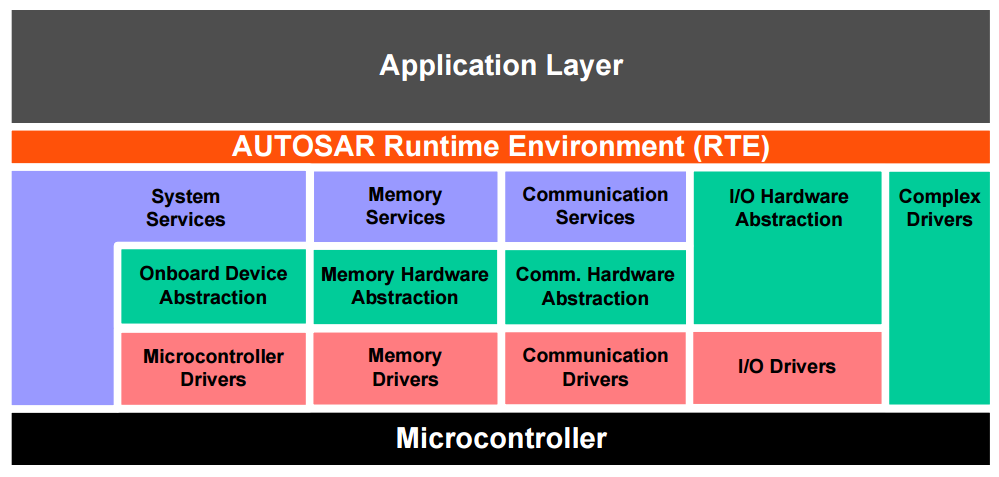
\includegraphics[scale=0.35]{content/images/autosararch.png}
	\caption{AUTOSAR Architecture \cite{autosararch}}
	\label{fig:autosararch}
\end{figure}
\section{Multi-core Programming with XMOS Multi-core Microcontrollers}
Some text will come here! \\
\section{Multi-core Programming with Raspberry Pi 3}
Some text will come here! \\
%%% CHAPTER Multi-core Programming ------------------end----
%%% CHAPTER APP4MC Development Environment ----------begin----
\chapter{APP4MC Development Environment}
\section{Introduction} %Motivation
\section{Features}
\section{Modeling}
%%% CHAPTER APP4MC Development Environment ------------end----
%%% CHAPTER A4MCAR ----------------------------------begin----
\chapter{Distributed Multi-core Demonstrator (A4MCAR) Design and Implementation}
\section{System Overview}
As introduced in the Introduction chapter, A4MCAR is a demonstrator RC-Car for the APP4MC development environment. A4MCAR provides a distributed multi-core architecture that allows the demonstration of embedded low-level and high-level applications. Pictures of the A4MCAR can be seen in Figure \ref{fig:a4mcar}.
\begin{figure}[!ht]
	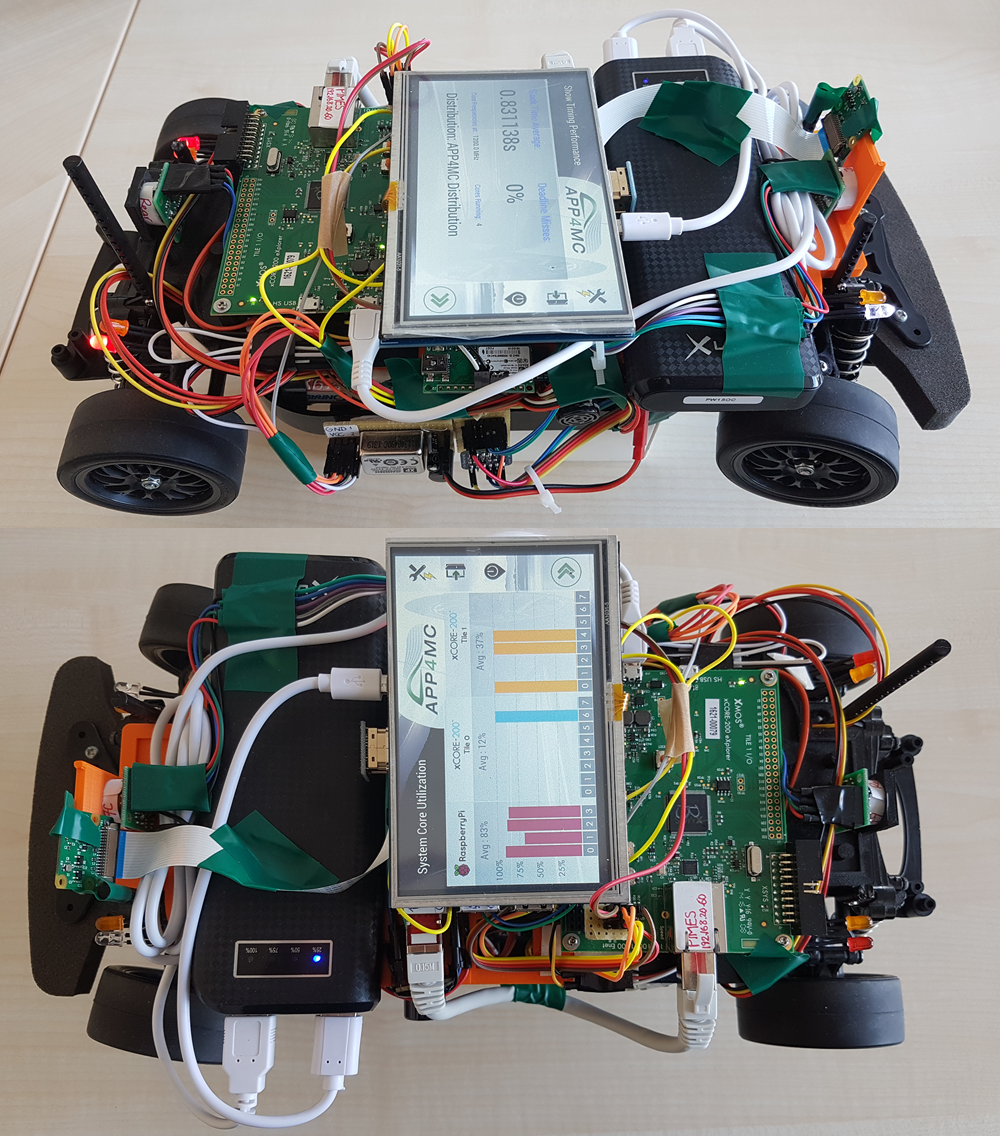
\includegraphics[scale=0.4]{content/images/a4mcar.png}
	\caption{A4MCAR}
	\label{fig:a4mcar}
\end{figure}
\subsection{System Features}
As A4MCAR targets automotive industry and parallelization studies done by APP4MC, it features not only sensing and actuation related features but also applications that would help with task to core distributions and parallelization performance evaluation. One could see the featured applications for the A4MCAR in Figure \ref{fig:tasksoverall}. 
\begin{figure}[!ht]
	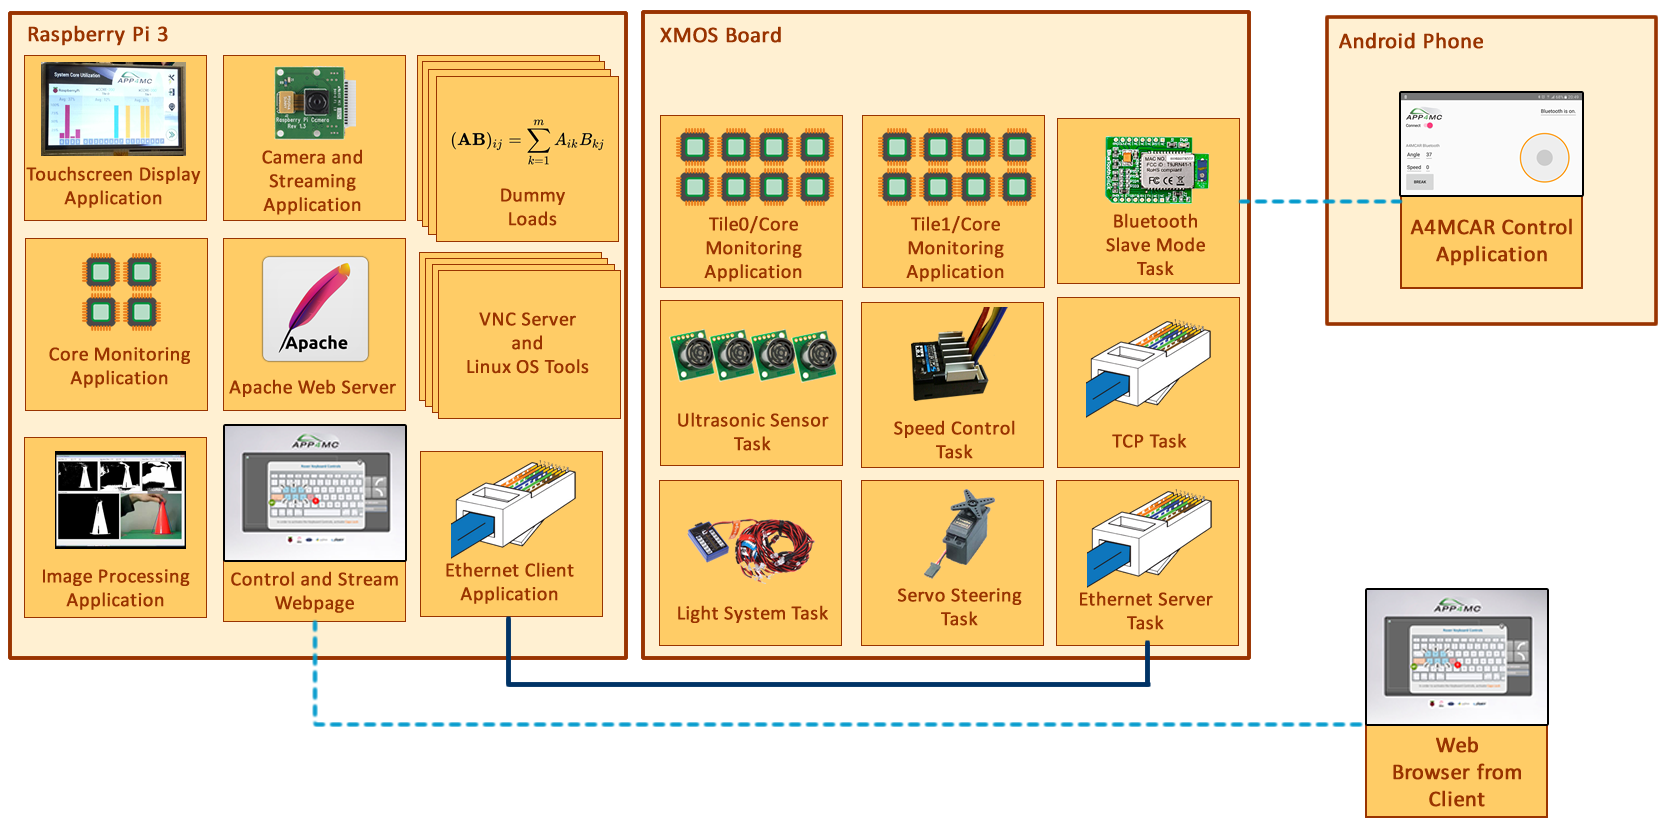
\includegraphics[scale=0.3]{content/images/tasksoverall.png}
	\caption{Applications developed and/or maintained for A4MCAR}
	\label{fig:tasksoverall}
\end{figure}
In the figure, it is seen that the low level module of A4MCAR, built using xCore-200 eXplorerKIT targets mostly actuation and sensing related applications. The full list of tasks developed for the low-level module includes:
\begin{itemize}
	\item Core monitoring applications for each tile (two exist) that calculates the average core usages.
	\item Bluetooth task to configure bluetooth module in slave mode and receive data over UART interface.
	\item Proximity measurement task that obtaines the distance sensor information from four SR-04 sensors over an I2C sensor network.
	\item Speed control task in order to use PWM to drive speed controlling motor.
	\item Steering task that controls a servo motor using PWM signaling in order to steer the A4MCAR using external inputs.
	\item Light system task in order to control a light module for certain conditions.
	\item Ethernet server task to maintain a TCP server for data reception and transmission from high level module.
	\item TCP task and several other ethernet configuration related tasks to configure ethernet module (PHY) drivers and establish proper TCP connection.
\end{itemize}
In order to investigate parallelization outcomes on Real-time Linux and make use of high level features such as web server, image processing and touchscreen interface high-level module is introduced to the system. High-level module is designed so that it can communicate with low-level module over TCP in order to send driving information and retrieve core information from low-level module. It is important to mention that high-level module uses Raspberry Pi 3 in order to achieve high level tasks using a robust Debian-based OS, namely Raspbian. Although the features of the high-level module is illustrated in the Figure \ref{fig:tasksoverall}, full feature list can be given as follows:
%xxxxxxxxxxxxxxxx
\begin{itemize}
	\item Core monitoring application that calculates the average core usages on each core.
	\item Image processing application that helps to find a traffic cone.
	\item Apache Web Server that is used to host a web page which shows average core usage, show Raspberry Pi 3 camera (Raspicam) stream and helps to drive the A4MCAR via web page controls.
	\item Ethernet client application that writes handles data transmission and reception to and from server using file operations and data parsing.
	\item Camera and streaming application that starts the Raspicam and maintains the stream using configuration parameters such as resolution, quality, frame rate, port and etc.
	\item A webpage which is used for driving the A4MCAR as well as display core usages on each core and Raspicam stream.
	\item A touchscreen display application which is used for displaying all cores and their utilization, starting and killing all applications on high-level module, allocation of processes on high-level module to cores dynamically, visualization of timing related performance indicators such as average slack time and deadline misses percentage, selecting different distributions, and configuration of the IP addresses on high-level module.
	\item Dummy load processes that perform random matrix multiplication in order to find performance indicators in full utilization.
	\item Several Linux processes that run Linux OS kernel and VNC server process that provides PC connection via SSH connection.
\end{itemize}
\subsection{Infrastructure}  %x XMOS and Rpi: boards, (inkl. board pictures) processors, memory, languages, compilers, infrastructure
Processing infrastructure of the A4MCAR is divided into two modules: Low-level module and high-level module. Low-level module uses a multi-core development kit XMOS xCore-200 eXplorerKIT, whereas high-level module uses a Raspberry Pi 3 which are both shown in Figure \ref{fig:boards}.
\begin{figure}[!ht]
	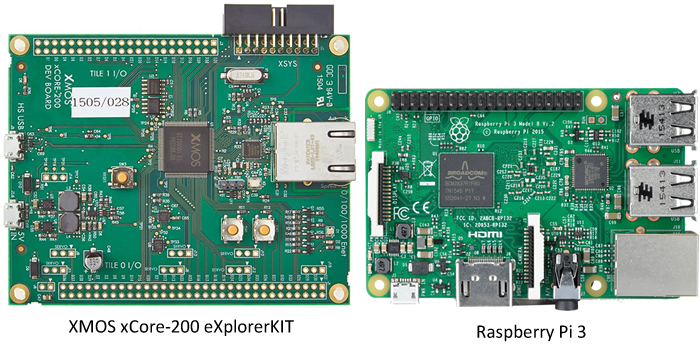
\includegraphics[scale=0.6]{content/images/boards.jpg}
	\caption{Development boards used in A4MCAR}
	\label{fig:boards}
\end{figure}

\subsubsection{Low-level Infrastructure}
XMOS xCore-200 eXplorerKIT features XEF216-512, a powerful multi-core microcontroller that provides sixteen 32-bit logical cores that are divided into tiles \cite{xmoskitweb}, which are identical units that contain processing unit, cache memory and switch mechanism \cite{tileref}. XMOS xCore-200 eXplorerKIT contains two tiles with eight logical cores in each tile. It is important to add that logical cores of eXplorerKIT provides 2000 MIPS (Million Instructions per Second) processing power and 512 KB SRAM along with up to 500 MHz clock speed. The specified performance values are considered to be relatively powerful compared to regular microcontrollers. While the processing power and cache memory of its two tiles are identical, ports on each tile have access to different peripherals located on the board. With 53 high-performance GPIO, XMOS xCore-200 eXplorerKIT features 100/1000Mbps Ethernet module, high speed USB interface, a 3D accelerometer, a 3-axis gyroscope, and six servo interfaces which makes the kit useful in a wide variety of applications that include robotics, automotive, signal processing and communication applications \cite{xmoskitweb}.

As the name of the development kit suggests, XEF216-512 uses XMOS' xCore-200 architecture. An illustration of xCore-200 architecture is given in Figure \ref{fig:XE216Architecture}.
\begin{figure}[!ht]
	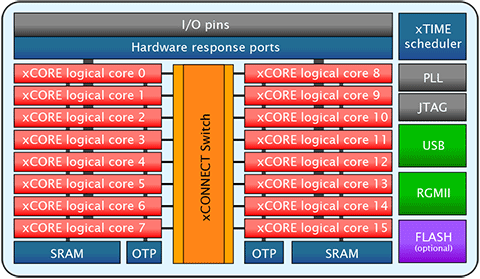
\includegraphics[scale=0.7]{content/images/XE216Architecture.png}
	\caption{Illustration of XMOS' xCore-200 Architecture \ref{fig:XE216Architecture}}
	\label{fig:XE216Architecture}
\end{figure}

In xCORE-200 architecture, each core uses the memory of the tile it belongs to and logical cores communicate using a high-speed network. Thus, channels which achieves task communication are linked to other cores via \textbf{xCONNECT Switch}. While this is the case for tasks that are distributed to seperate cores, for tasks that are placed in the same core \textbf{xTIME Scheduler} automatically schedules tasks by synchronizing events. The xTIME Scheduler works similar to RTOS in traditional microcontrollers and uses \textbf{Round-robin scheduling method} \cite{xmosdatasheet} \cite{roundrobin} which is a simple and starvation-free scheduling technique that gives each task equal time slices and disregards priorities in order to schedule processes or tasks. Round-robin scheduling is widely used in operating systems \cite{roundrobin}.

In xCORE architecture, the synchronization of task communication is handled by events rather than ISRs (Interrupt Service Routines) as compared to a traditional microcontroller. Each xCORE tile is connected to hardware ports and thereby pins which can be driven high and low in order to drive electrical peripherals. xCORE tiles are also connected to an OTP (One Time Programmable Memory) and SRAM (Static Random Access Memory). While OTP is used for code locking features, SRAM serves as a memory where the instructions and variables are located \cite{xmosdatasheet}.

Since the xCORE features multiple cores unlike a traditional microcontroller, it should be clearly understood that the task interruption is not present in xCORE. This is illustrated delicately in the Figure \ref{fig:xmosvstraditional} \cite{xmosflyer}. If not stated otherwise in an xCORE application, all the tasks are placed to different logical cores. This means that all the tasks are executed completely parallel in hardware. When the tasks are shared in a core, then the multi-tasking features of the XMOS are invoked and parallelized just like in an RTOS from traditional microcontrollers \cite{xmosflyer}.
\begin{figure}[!ht]
	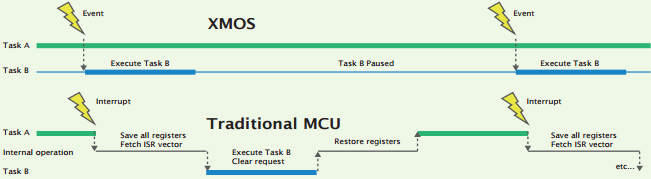
\includegraphics[scale=0.72]{content/images/xmosvstraditional.png}
	\caption{XMOS vs Traditional Microcontroller \cite{xmosflyer}}
	\label{fig:xmosvstraditional}
\end{figure}

Most of the traditional microcontrollers including xCORE microcontrollers nowadays feature pipelining mechanism. The \textbf{instruction pipeline} is a set of data processing elements connected in series, where the output of one element is the input of the next one \cite{pipelinebook}. Via instruction pipelining, processors make use of the stages in order to use the clock to its full performance to reduce the time taken to execute instructions. This mechanism is also present in most of the XMOS processors with five stages. How instruction pipelining mechanism achieves faster instruction execution is illustrated in the Figure \ref{fig:pipeline} \cite{xmosflyer}.
\begin{figure}[!ht]
	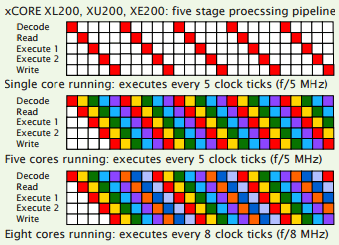
\includegraphics[scale=0.9]{content/images/pipeline.png}
	\caption{Pipelining Explained on XMOS \cite{xmosflyer}}
	\label{fig:pipeline}
\end{figure}

Traditionally, XMOS based microcontrollers are programmed via xTimeComposer, which is an Eclipse-based software development platform for XMOS based multi core microcontrollers with integrated features such as simulation, symbolic debugging, tracing, runtime instrumentation, and timing analysis with a static code timing analyzer called \textbf{XTA}\cite{xmosflyer}. As A4MCAR needs to make use of timing and performance values, some tracing tools and XTA has been widely used during the development. xTIMEComposer development environment windows are shown and illustrated in Figure \ref{fig:xtimecomposerwindows}.
\begin{figure}[!ht]
	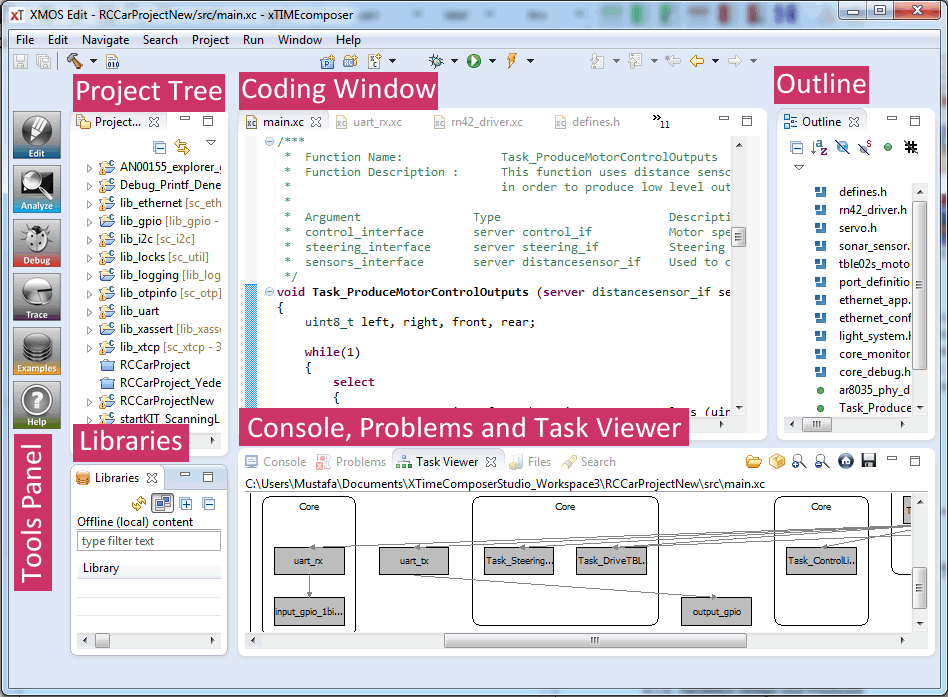
\includegraphics[scale=0.5]{content/images/xtimecomposerwindows.png}
	\caption{xTIMEComposer 14.2.3 Development Environment Windows}
	\label{fig:xtimecomposerwindows}
\end{figure} \\
%Explain the fucking composer
In the Figure \ref{fig:xtimecomposerwindows} it is seen that the main development environment consists of the following windows:
\begin{itemize}
	\item \textbf{Project Tree:} This window is used for managing projects and source, include, binary and configuration files within projects.
	\item \textbf{Coding Window:} Coding window is used for writing code and placing breakpoints. One can switch between several files by clicking on the tabs located on the top of this window.
	\item \textbf{Console:} The console is used for viewing the building process, verbose and debugging information.
	\item \textbf{Problems:} The problems window is used for seeing warnings and errors that result from the code.
	\item \textbf{Task Viewer:} The task viewer is a special feature that is unique in xTIMEComposer and it is used to visualize tasks and at which core and tile they are located. The channel and interface connections between tasks are also visualized using this window.
	\item \textbf{Tools Panel:} This window is used in order to switch between several tools that xTIMEComposer provide. Analyze and Debug tools are widely used in development. Analyze tool opens xTIMEComposer Timing Analyzer (XTA) tool whereas Debug tool is used for traditional debugging using breakpoints.
	\item \textbf{Outline:} Outline window lays out the main elements of a file such as its includes, tasks, objects and so on.
	\item \textbf{Libraries:} The Libraries window can be used in order to search offline and online libraries.
\end{itemize}
%files in a project.. configuration..
%\begin{figure}[!ht]
%	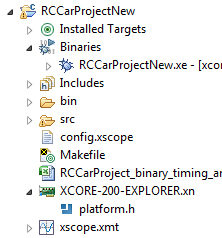
\includegraphics[scale=0.9]{content/images/xtimeprojecttree.jpg}
%	\caption{Files in a xTIMEComposer project}
%	\label{fig:xtimeprojecttree}
%\end{figure}
%languages
Programming languages which are used for xCORE processors can be listed as C, C++ and xC (C with multicore extensions) \cite{xmosdatasheet}. The aforementioned xC language features three main keywords in order to represent task communication. To represent an interface that sends data to another task, \textbf{client} keyword is used whereas if a task is retrieving data from one or many client ports, the receiving interface is named \textbf{server}. It is important to mention that server interface receives data by throwing events. Additionally, xC also allows to define function attributes which are \textbf{combinable} and \textbf{distributable}. XMOS Programming Guide \cite{xmosprogrguide} suggests that combinable tasks are the ones that continuously react to events and they can be combined to have several tasks running on the same logical core. It is added in the XMOS Programming Guide \cite{xmosprogrguide} that distributable tasks are not dedicated to only one logical core but they run when required by the tasks connected to them. Furthermore, xC features \textbf{timers}, \textbf{events}, \textbf{guards}, \textbf{event priority ordering} in order to help us develop event-based software. These features of xC make multi-core programming easy and robust on xCORE processors.

\subsubsection{High-level Infrastructure}
%xxxxxxxxxxxxxxxx
High-level processing unit of A4MCAR, Raspberry Pi 3, is a widely used single board computer in embedded applications. It has 1.2GHz 64-bit quad-core processor with ARMv8 architecture, 1GB of RAM, VideoCore IV 3D graphics core and several interfaces such as 40 GPIO pins, 4 USB ports, HDMI port, ethernet port, audio jack, camera interface (CSI), display interface (DSI), micro SD card slot \cite{raspberrypiinfo}. The reason Raspberry Pi 3 is preferred in embedded systems applications is that it provides excellent connectivity via 802.11n Wireless LAN module, Bluetooth 4.1 module, and Bluetooth Low Energy (BLE) module. 

Raspberry Pi 3 can be booted with modern Linux-based operating system distributions such as Debian-based Raspbian OS \cite{raspbiandownload} and Ubuntu-based Ubuntu MATE\cite{ubuntumatedownload} \cite{raspberrypiinfo}. It should be noted that in A4MCAR, Raspbian OS has been used due to its wide software repository and driver support. The fact that Raspberry Pi 3 functions as a Linux computer helps in developing high-level applications that require operating system presence. The open-source nature of Linux and its software ecosystem provides flexible and traceable software development. In A4MCAR, the traceability and flexibility features of Raspberry Pi 3 are highly used. Furthermore, a wide variety of programming languages such as C, C++, Java, LISP, Python, Bash, Perl etc. are supported in Raspberry Pi. In A4MCAR, programming languages such as C, C++, Python, Bash, HTML, JavaScript has been used in order to develop high-level module.

A brief explanation of the architecture of Linux-based computers and as an extension the architecture of the Raspberry Pi 3 should be given in order to develop applications and understand how applications running on Linux work. With that idea in mind, high-level overview of the structure of  the \textbf{Linux kernel} and high-level layers in a Linux system which is given in Figure \ref{fig:linuxarchitecture} should be considered \cite{linuxkernelbook}.
\begin{figure}[!ht]
	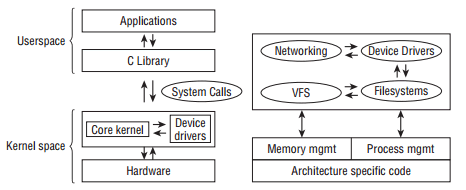
\includegraphics[scale=0.9]{content/images/linuxarchitecture.png}
	\caption{High-level Linux system architecture \cite{linuxkernelbook}}
	\label{fig:linuxarchitecture}
\end{figure}

According to Mauerer \cite{linuxkernelbook}, the kernel is the intermediary level between the hardware and the software that addresses the devices and the components of the system (such as CPU, memory and I/O devices) by passing application requests. While kernel processes requests from user applications, it makes its own decision where data is located and which commands to send to hardware. Kernel is also the instance in a Linux system which shares available resources such as CPU, memory, and network; which is why it should be addressed while working with parallel applications.

In the figure, it is seen that kernel space is not only responsible for accessing device drivers, but it is also responsible for memory and process management. A program under Unix systems (such as Linux) that run continuously is referred to as \textbf{processes} and they are scheduled by Linux kernel. The multi-tasking of processes are done by a mechanism that is called \textbf{task-switching} or \textbf{context-switching} and this is achieved to ensure that CPU performs according to the scheduled tasks. The concept of \textbf{scheduling} in a Linux system is also handled by kernel and it is the procedure of deciding how CPU time should be shared between existing processes. Additionally, \textbf{threads} in a Linux-based computer system are also big parts of multi-tasking which are also handled by kernel. Threads share the same data and resources but they have different execution paths through program \cite{linuxkernelbook}.

In A4MCAR high-level module, we mostly deal with processes and investigate ways to efficiently parallelize process-based system. In this regard, it is crucial to understand the process life cycle and how kernel schedules processes. This knowledge is described delicately by Mauerer \cite{linuxkernelbook} and Ward \cite{howlinuxworksbook}. Figure in \ref{fig:processlifecycle} depicts an illustration of how process life cycle works \cite{linuxkernelbook}.
\begin{figure}[!ht]
	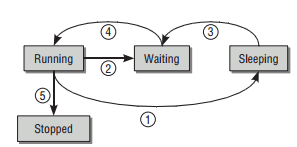
\includegraphics[scale=1]{content/images/processlifecycle.png}
	\caption{Process Life Cycle in a Linux System \cite{linuxkernelbook}}
	\label{fig:processlifecycle}
\end{figure}

% process life cycle explain..
In Figure \ref{fig:processlifecycle}, state machine for processes in a Linux system is given. The states of processes can be listed as Running, Waiting, Sleeping, and Stopped. These states can be explained using following scenerios \cite{linuxkernelbook}:
\begin{itemize}
	\item If the process is being currently executed, process is in \textbf{Running} state.
	\item If the process is not being executed because it is waiting for CPU to finish executing another process, it is in \textbf{Waiting} state.
	\item If the process is waiting for an external event such as a periodic activation or a sporadic activation, it is in \textbf{Sleeping} state. Notice that transition from Sleeping state to Running state is not possible. A process switches to Waiting state from Sleeping state in order to wait for current process to finish its execution.
	\item If the user decides to kill (terminate) the application, the process goes into \textbf{Stopped} state.
	\item If a process has been killed but its entries are still alive in the process table, the state of that process is called \textbf{Zombie}. Therefore, although not shown, transition from Running state to Zombie state is also possible.
\end{itemize}

It is important to note that these states are traceable using Linux kernel access methods which will be explained in Section 5: "Information Tracing and System Management" of this report along with several other Linux kernel concepts.

% terminal, compilers, Nano, Vi, Emacs
Raspberry Pi is conventionally programmed through Linux shell which is programmed and commanded with the help of Bash scripting language. There are several editors and compilers introduced for Linux shell in order to help developers write, compile, debug, and trace their applications. Most popular editors involve Nano, Vi, and Emacs which are editors that can run without GNU Graphical User Interface. An alternative way is to use open-source platforms such as Eclipse with correct extensions and plugins. The conventional and standart C compiler for the Unix platform GCC, and the standart Python shell can be accessed using all these compilers. For the sake of demonstration, the Linux shell which is running Emacs is shown in the Figure \ref{fig:linuxeditors}. It is important to note that in the development of A4MCAR, Nano and Emacs editors have been frequently used as Nano provides easiest way to interact with Linux shell and Emacs provides advanced features to compile and debug programs rapidly.
\begin{figure}[!ht]
	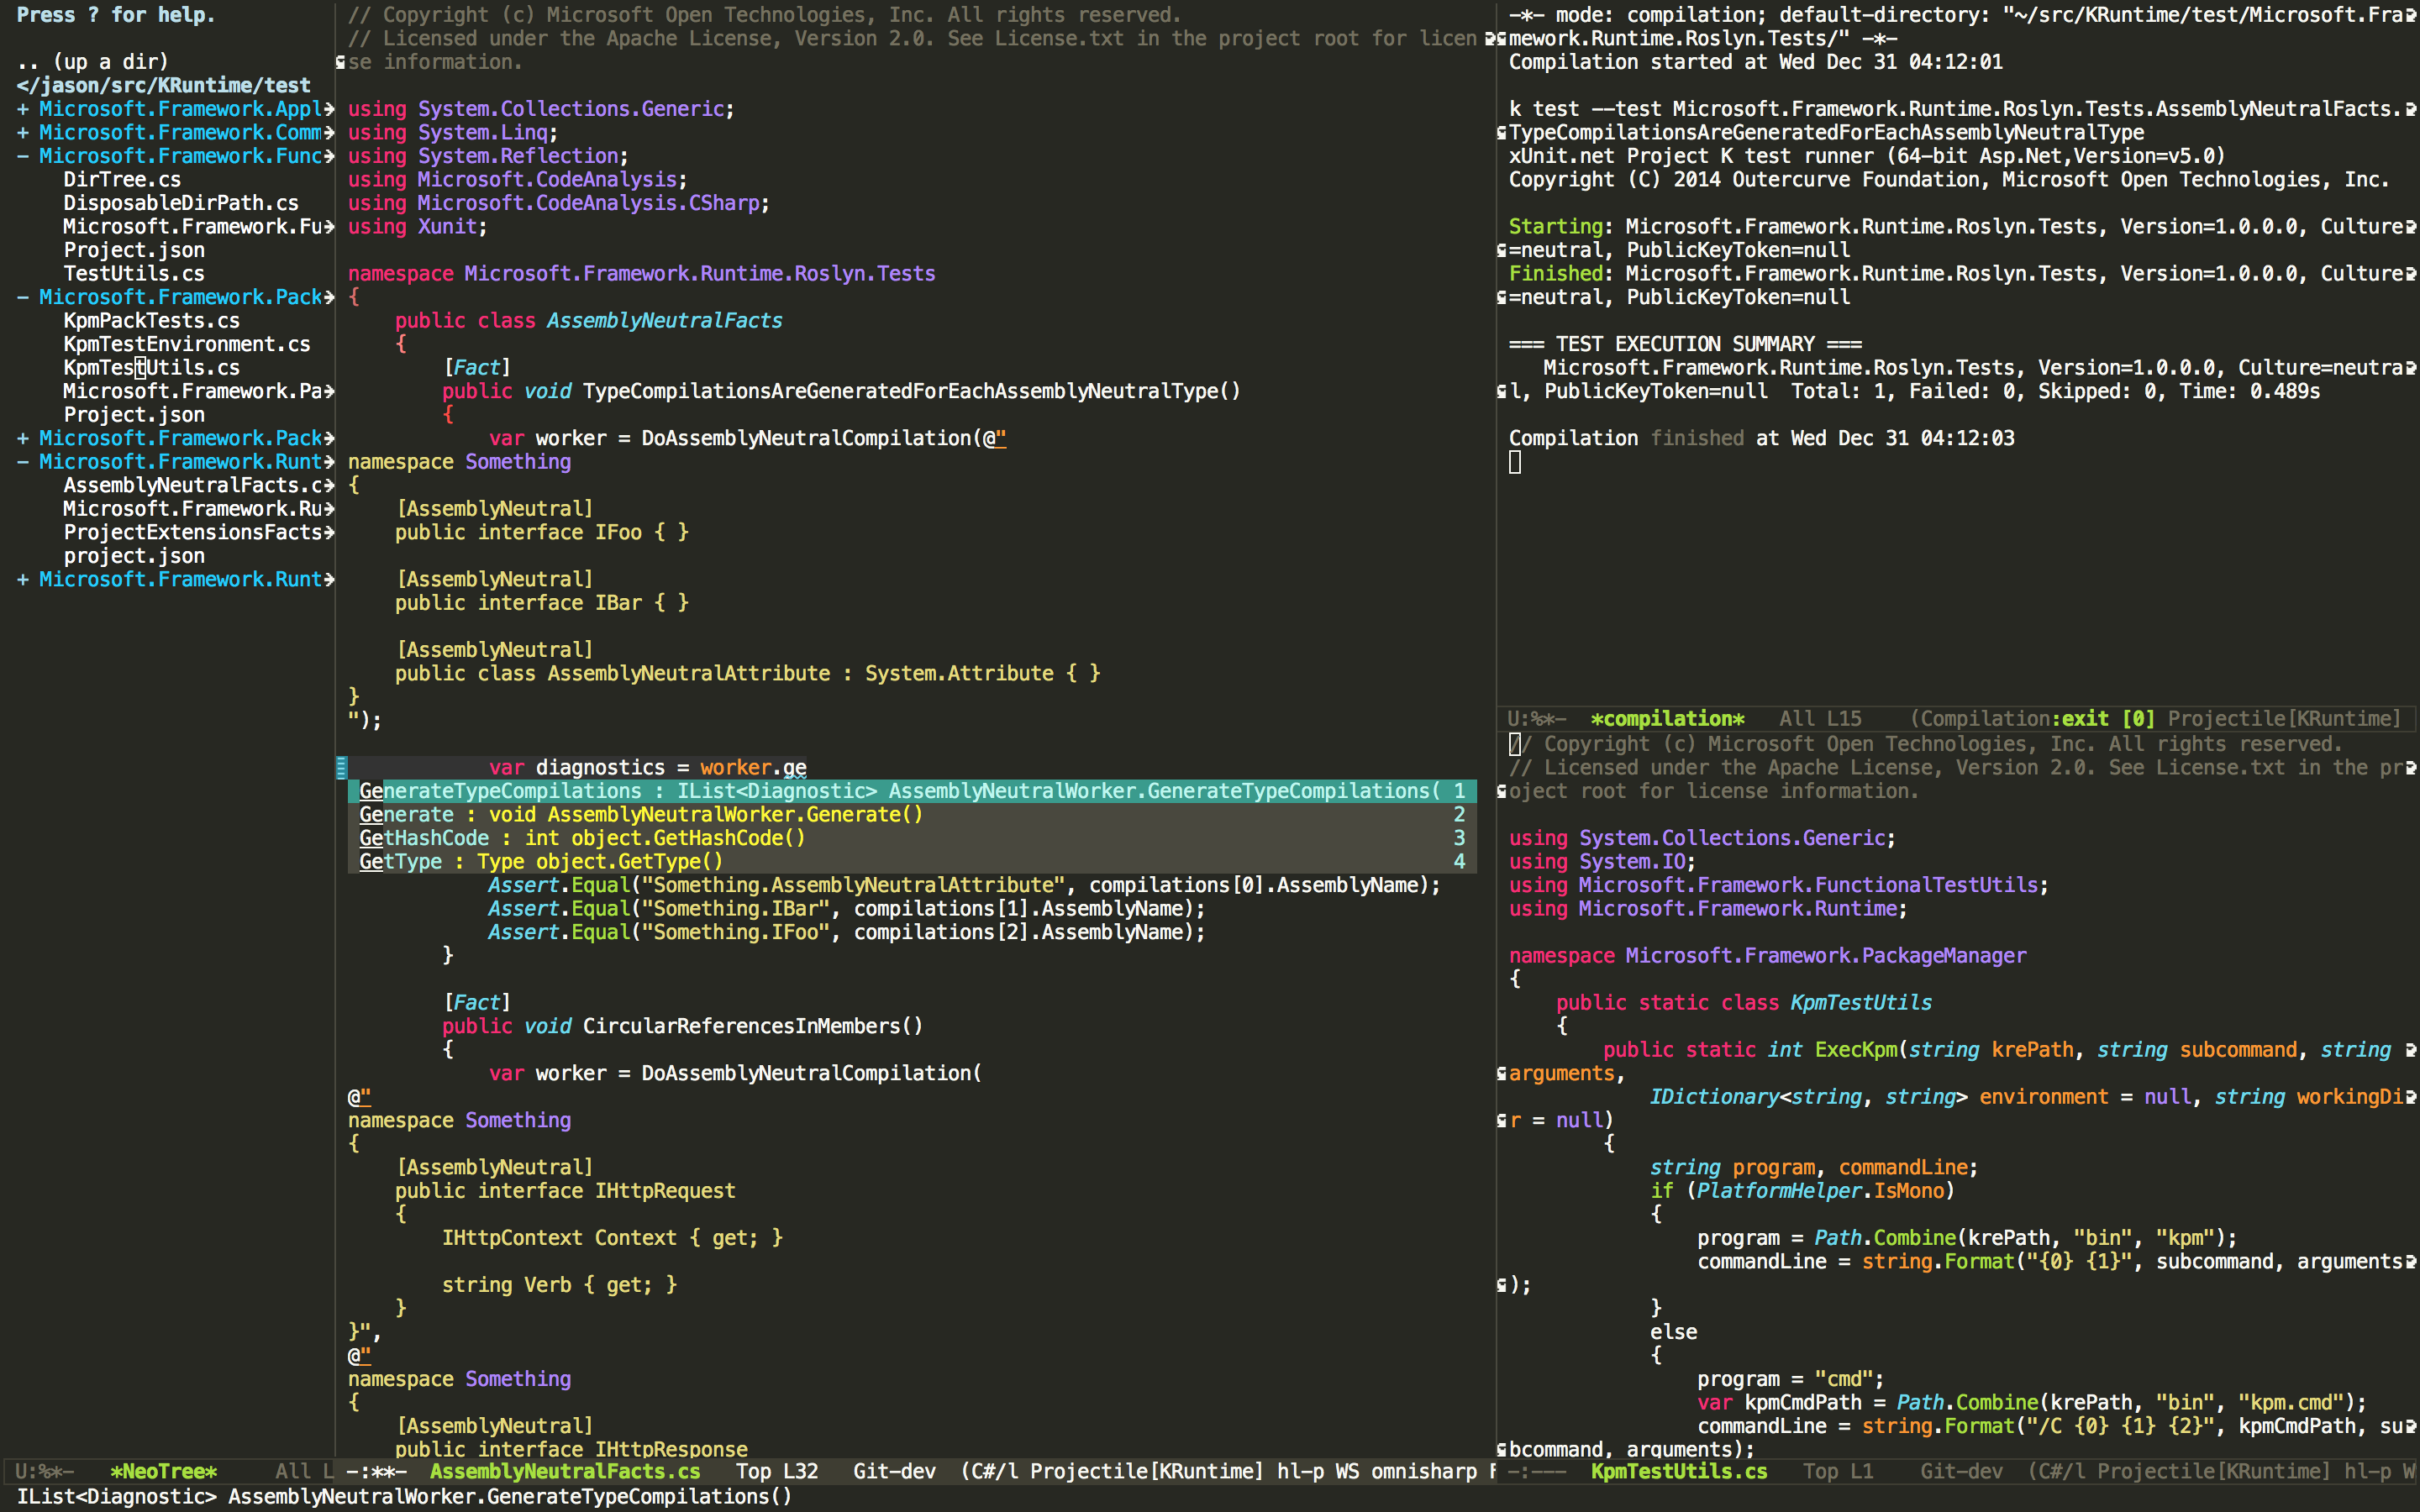
\includegraphics[scale=0.2]{content/images/linuxeditors.png}
	\caption{Linux Shell running Emacs}
	\label{fig:linuxeditors}
\end{figure}
%Raspbery Pi stuff here!
\subsection{Hardware Design, Sensors and Protocols}
One should care for a robust hardware design in order to avoid having software problem and safety related issues. In A4MCAR, a number of modules have been used alongside development kits in order to provide utility to the demonstrator. On the low-level module side, a light system, an RN-42 Bluetooth module, four SRF-02 ultrasonic sensors, a servo motor, a TBLE-02S electronic speed controller have been used. The high-level module side however only is connected to a touchscreen display and a Raspicam (Raspberry Pi camera). The overview of hardware connections, used protocols and device architectures are given in the Figure \ref{fig:hwoverview}.
\begin{figure}[!ht]
	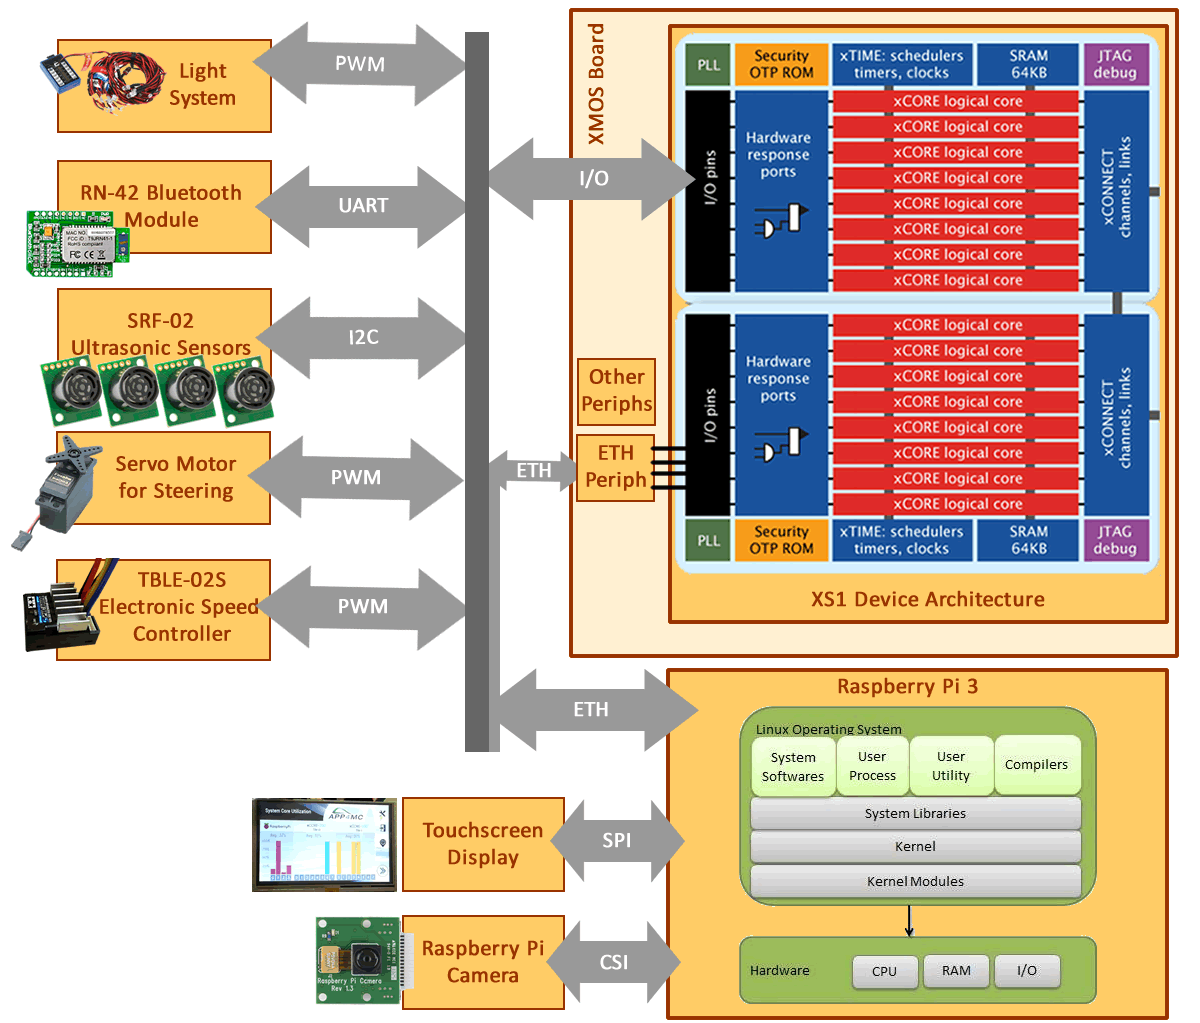
\includegraphics[scale=0.37]{content/images/hwoverview.png}
	\caption{Hardware overview of A4MCAR}
	\label{fig:hwoverview}
\end{figure}

The system uses various communication protocols, seen in Figure \ref{fig:hwoverview} in order to interact with sensors, actuators and utility devices. The communication protocols and associated devices used in A4MCAR could be listed as follows:
\begin{itemize}
	\item \textbf{PWM:} In order to interact with servo motor, TBLE-02S electronic speed controller, and light system, Pulse Width Modulation (PWM) have been used. PWM is a type of modulated digital signal used mostly in control applications \cite{pwm}. By describing how much a signal is high and low with respect to time, duty cycle is measured which is given in percentage. One could observe the signal illustration given in \ref{fig:pwm} to see how commonly used duty cycles look like. In a control circuitry, by achieving various duty cycles, dimming a light or controlling the direction or speed of a motor is possible \cite{pwm}.
	\begin{figure}[!ht]
		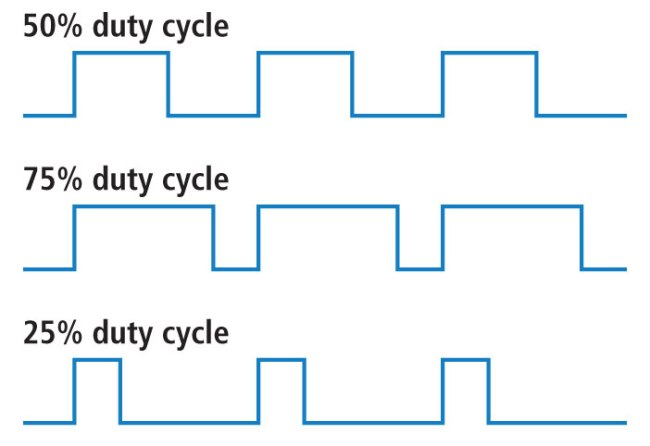
\includegraphics[scale=0.5]{content/images/pwm.jpg}
		\caption{Duty cycle example in pulse width modulation \cite{pwm}}
		\label{fig:pwm}
	\end{figure}
	\item \textbf{UART:} The RN-42 is a master-slave configurable bluetooth module (shown in Figure \ref{fig:hwoverview}) that is programmed using AT commands via UART. In A4MCAR, a RN-42 bluetooth module is used in order to interact with the bluetooth of Android devices. UART (Universal Asynchronous Receiver and Transmitter) is a communication protocol that achieves simple communication of two equivalent nodes. UART is a half-duplex and asynchronous serial protocol that doesn't communicate using a clock. Half-duplex nature of UART makes it so that transmitting and receiving lines can not be achieved simultaneously. It became a universal format because it is being used in telephone lines and USB ports of computers for decades. Number of bits transmitted or received per second is referred to as baud rate and it is standardized to values such as 9600, 14400, 19200, 38400, 57600, and 115200. Basic UART data packet is given in Figure \ref{fig:uartpacket}. The figure should depict that the basic format usually contains 6 to 8 data bits and start and stop bits to mark start and stop of the data packet. It should be noted that there are various formats with different sizes \cite{uart}.
	\begin{figure}[!ht]
		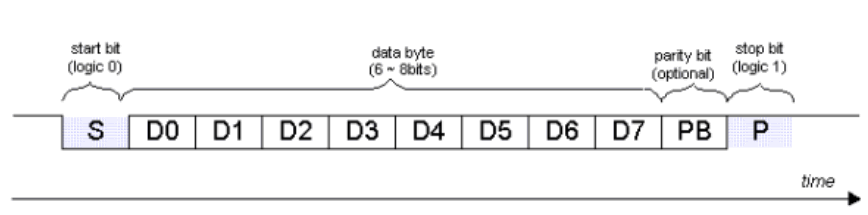
\includegraphics[scale=0.5]{content/images/uartpacket.png}
		\caption{Simple UART data packet \cite{uart}}
		\label{fig:uartpacket}
	\end{figure}
	\item \textbf{I\textsuperscript{2}C:} The proximity sensor network of A4MCAR that consists of four SRF-02 sonar sensors uses I\textsuperscript{2}C communication protocol in order to address devices in the network and obtain distance information in centimeters. I\textsuperscript{2}C (Inter integrated circuit) is a communication protocol that is intended for short distance that handles the communication of multiple slave units with one or multiple master units. Its advantage is that it uses only two wires in order to handle communication between many devices. Compared to the very similar serial communication protocol SPI, I\textsuperscript{2}C can support a multi-master system with up to 1008 slave devices. I\textsuperscript{2}C chips consist of two signals: clock signal SCL and data signal SDA. Since signals are open drain, each signal must have a pull-up resistor. The communication is handled by sending the address of the register and the data to be sent in order to write into the registers of the I\textsuperscript{2}C chips. A basic frame with 7 address bits and 8 data bits is given in \ref{fig:i2cframe} \cite{i2c}.
	\begin{figure}[!ht]
		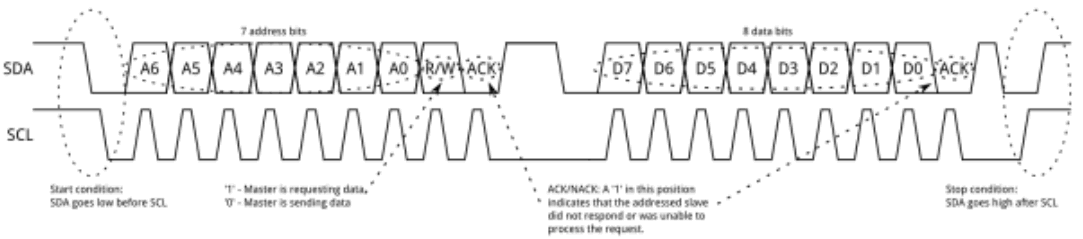
\includegraphics[scale=0.4]{content/images/i2cframe.png}
		\caption{I2C protocol frame\cite{i2c}}
		\label{fig:i2cframe}
	\end{figure}
	\item \textbf{Ethernet/TCP}:
\end{itemize}
\begin{figure}[!ht]
	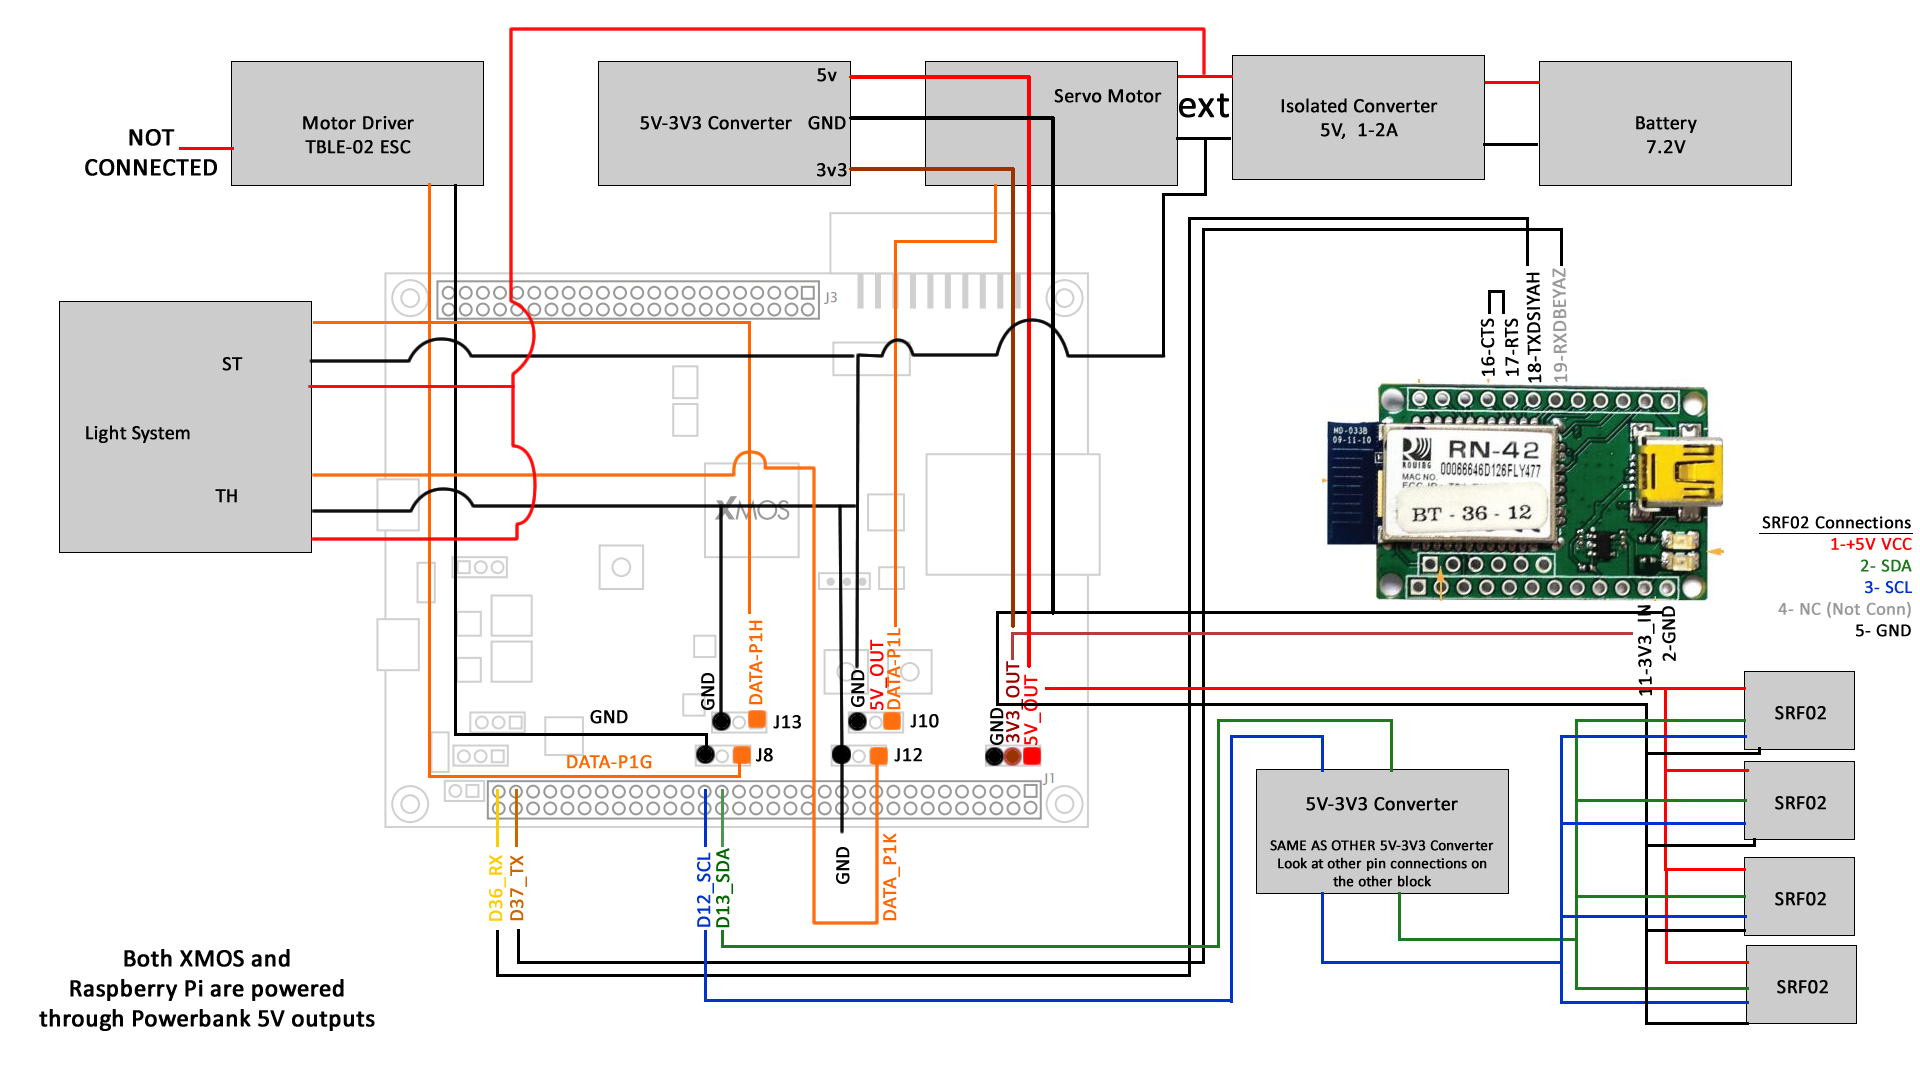
\includegraphics[scale=0.25]{content/images/RCCAR_Schematics.png}
	\caption{Low-level module schematics of A4MCAR using XMOS xCore-200 eXplorerKIT}
	\label{fig:RCCAR_Schematics}
\end{figure}
\subsection{Safety and Power}
Some text will come here! \\
\subsection{Mechanical Design}
Some text will come here! \\
\begin{figure}[!ht]
	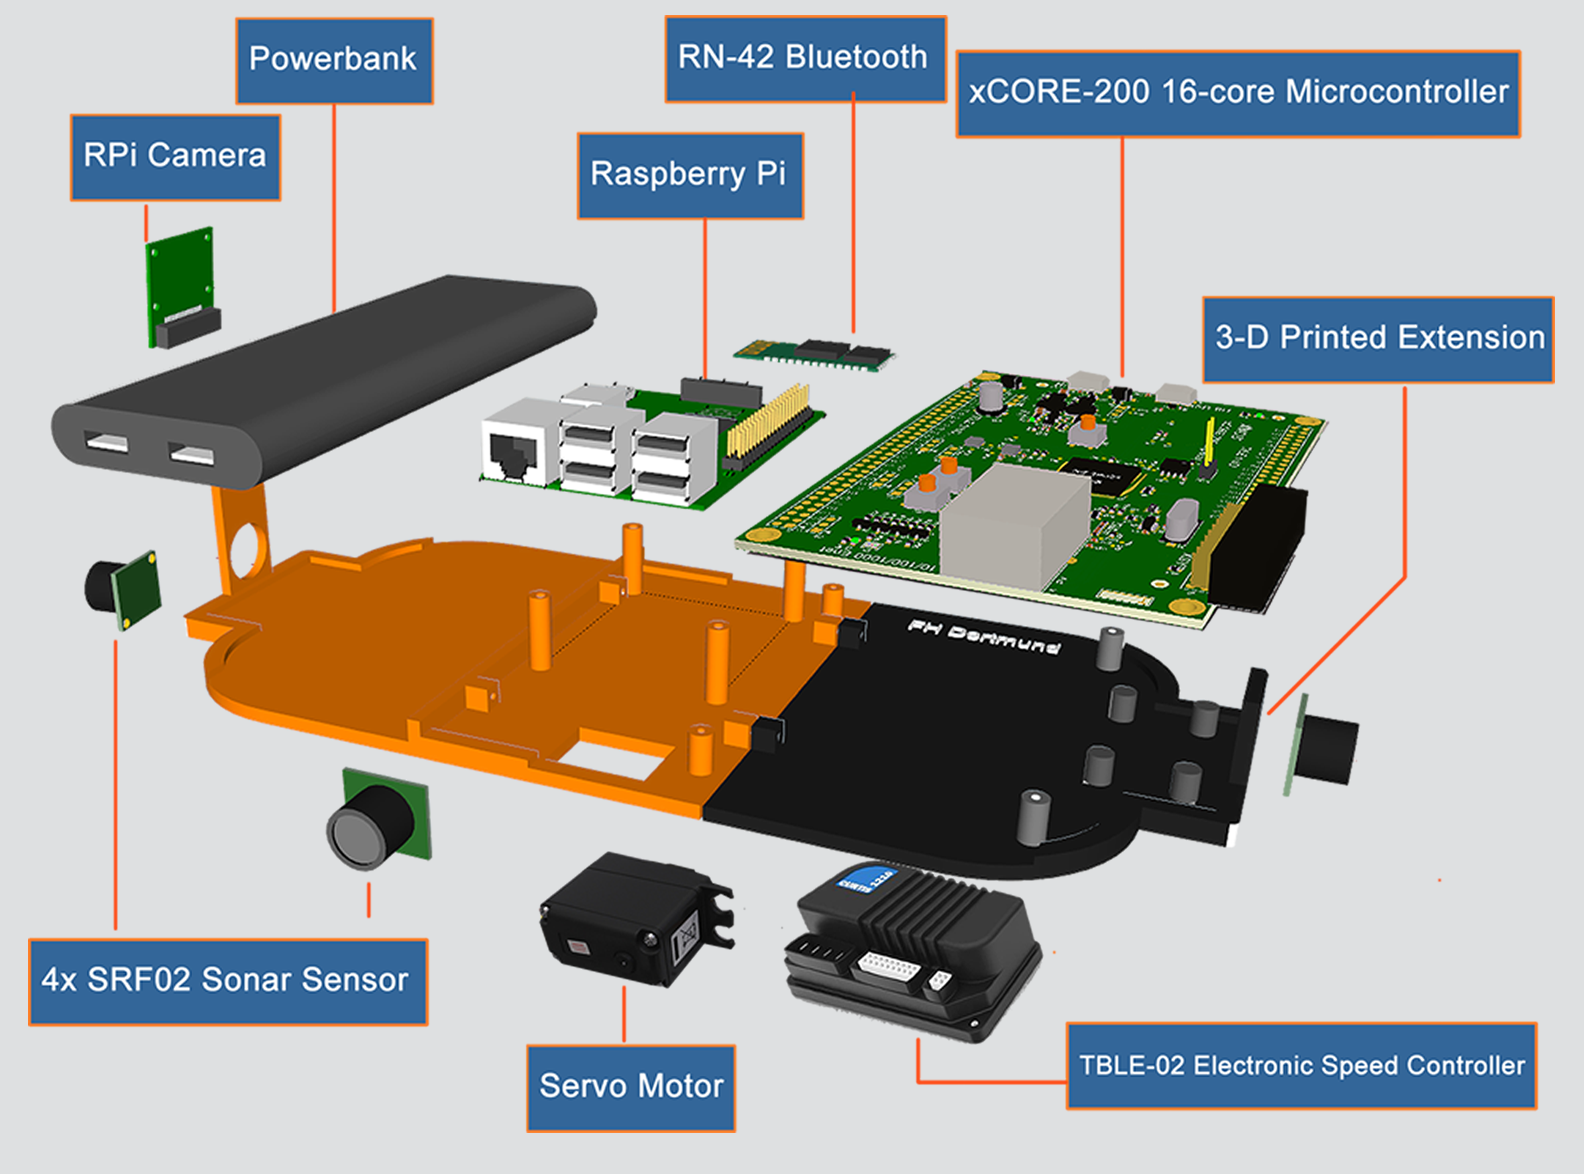
\includegraphics[scale=0.25]{content/images/mechanicaloverview.png}
	\caption{Mechanical overview of the A4MCAR}
	\label{fig:mechanicaloverview}
\end{figure}
\section{Low-Level Module Design and Implementation}
Some text will come here! \\
\subsection{Overview}
Some text will come here! \\
\begin{figure}[!ht]
	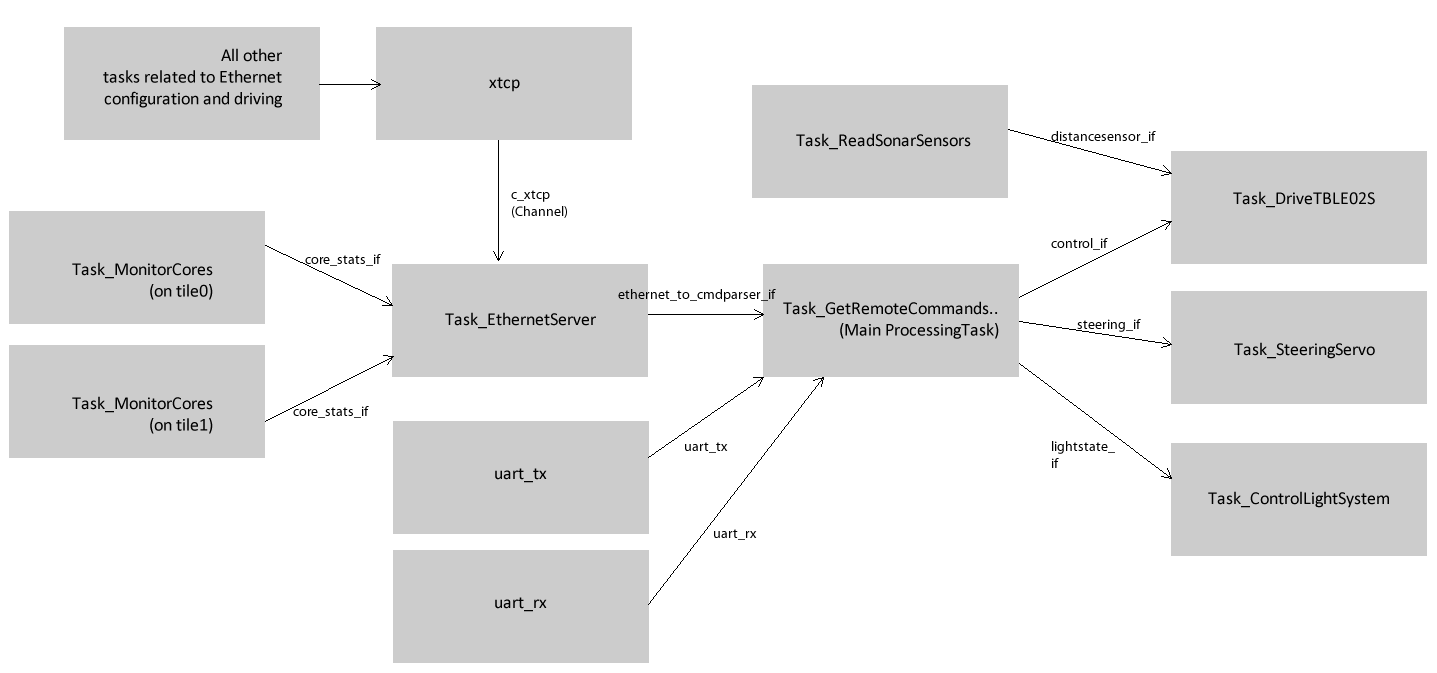
\includegraphics[scale=0.32]{content/images/sysmlxmostasksbrief.png}
	\caption{Brief block diagram for the developed tasks and interfaces for low-level module}
	\label{fig:sysmlxmostasksbrief}
\end{figure}
\begin{figure}[!ht]
	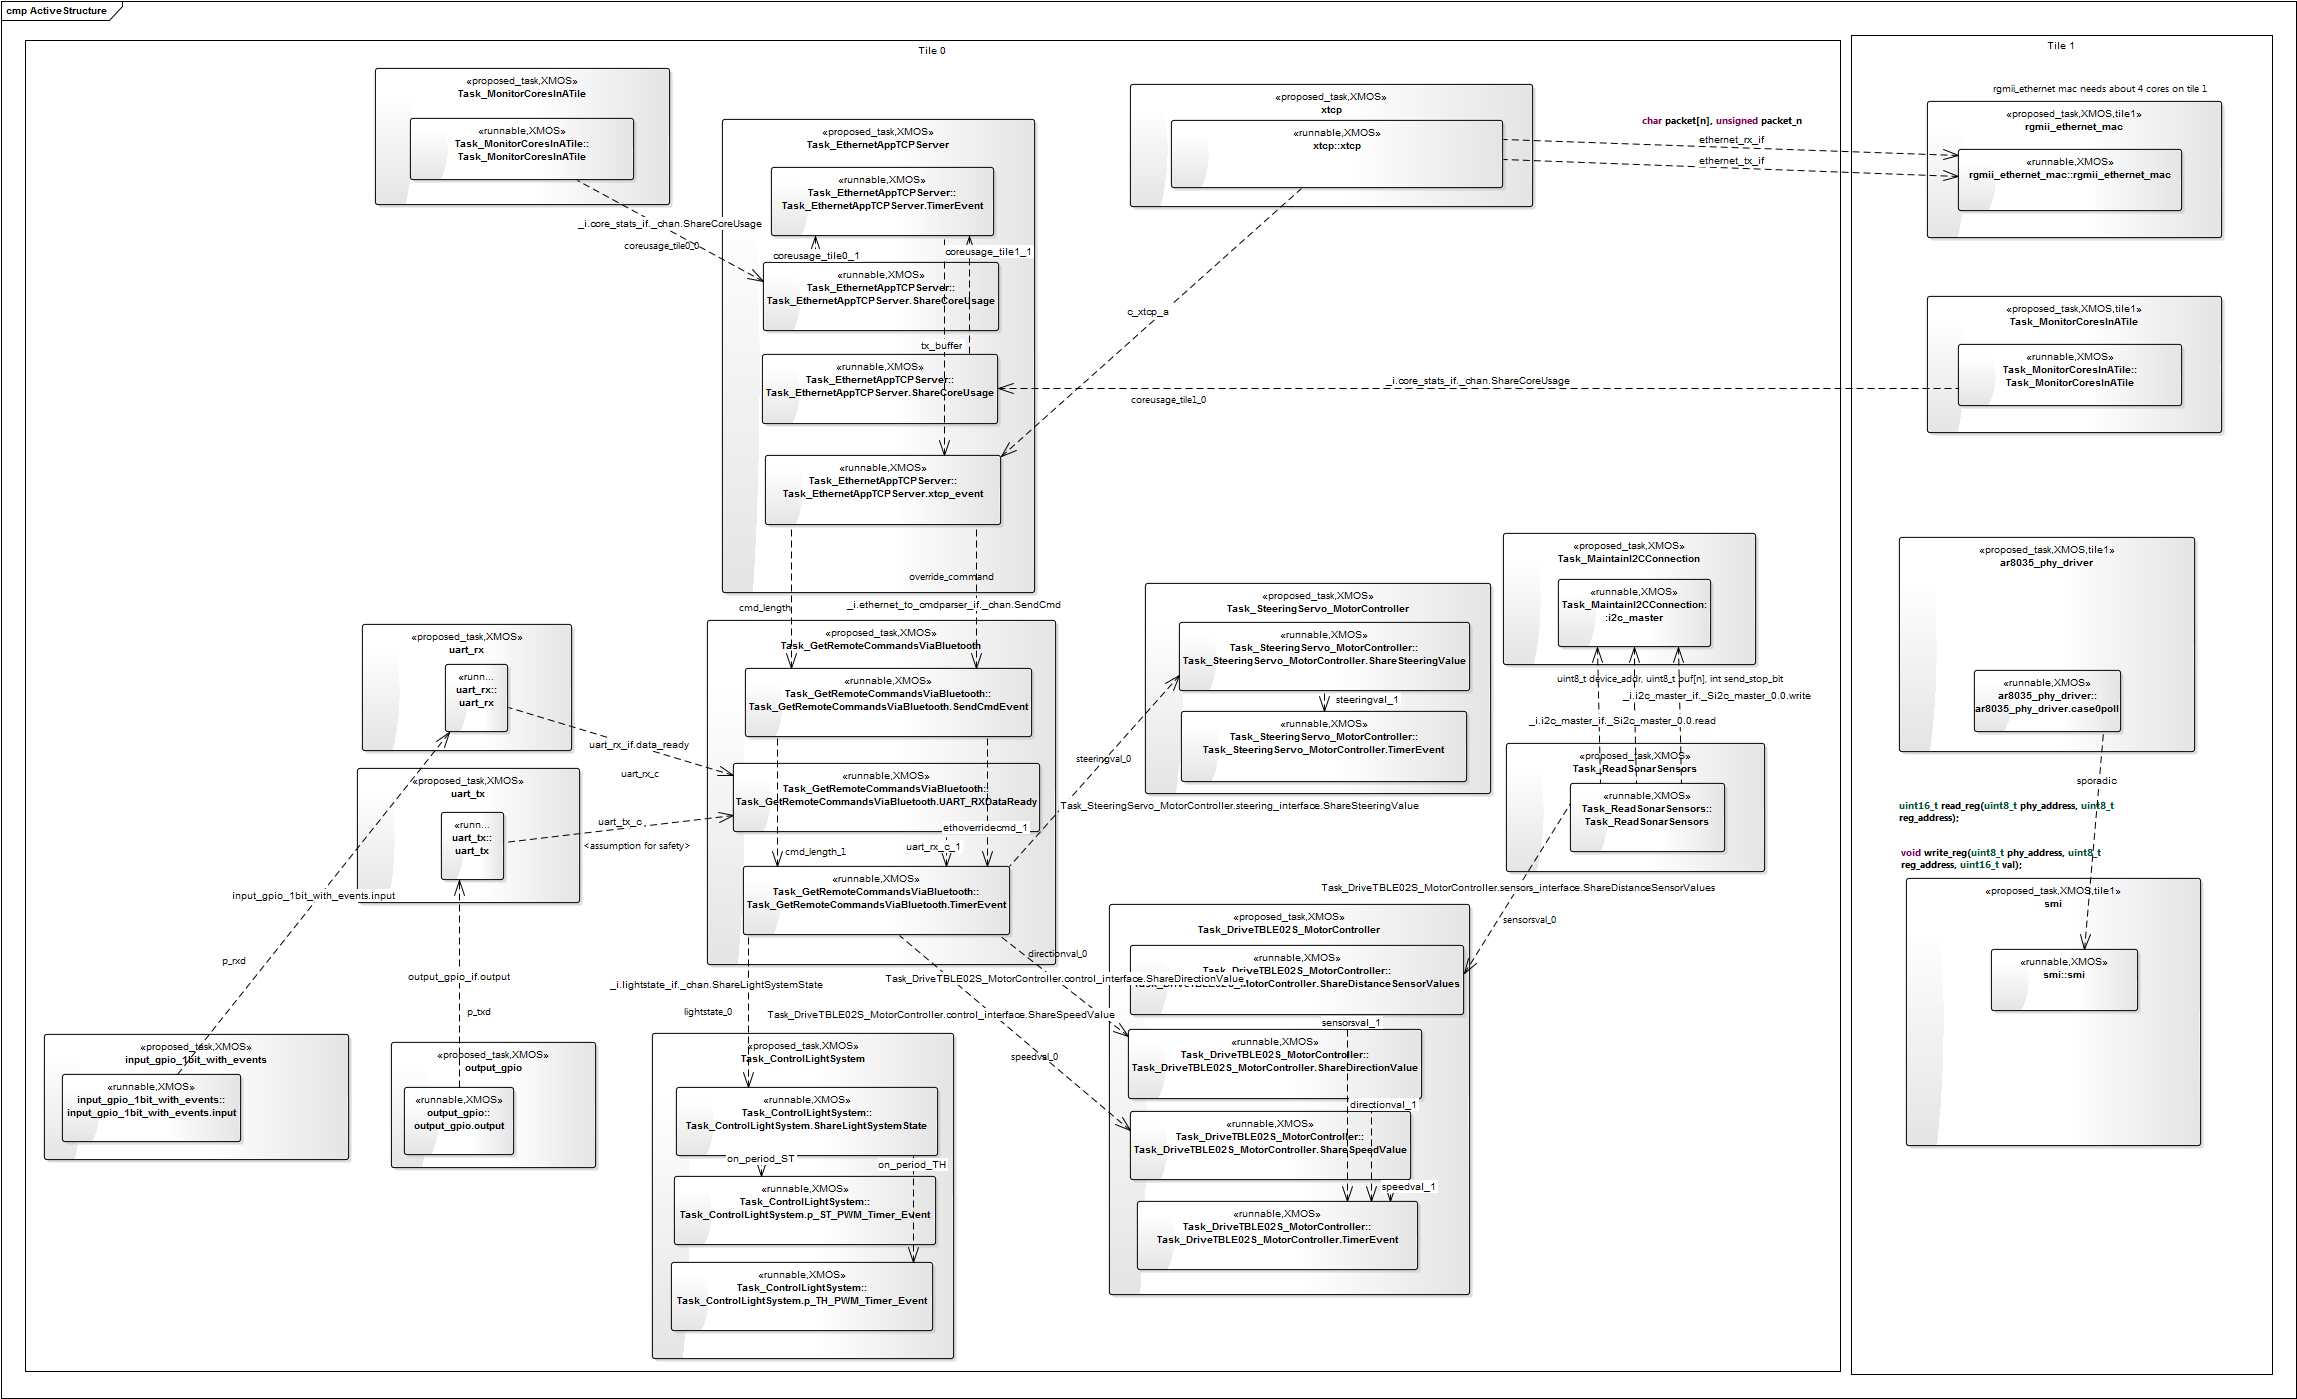
\includegraphics[scale=0.21]{content/images/sysmlxmostasks.png}
	\caption{Block diagram for the developed tasks and interfaces for low-level module}
	\label{fig:sysmlxmostasks}
\end{figure}
\subsection{Actuation}
Some text will come here! \\
\subsubsection{Acceleration}
Some text will come here! \\
\subsubsection{Steering}
Some text will come here! \\
\subsection{Proximity Sensing}
Some text will come here! \\
\subsection{Lighting System}
Some text will come here! \\
\subsection{Bluetooth Communication}
Some text will come here! \\
\subsection{Ethernet (TCP) Server Implementation}
Some text will come here! \\
\subsection{Core and Tile Monitoring}
Some text will come here! \\
\section{High-Level Module Design and Implementation}
Some text will come here! \\
\subsection{Overview}
Some text will come here! \\
\subsection{Core Monitoring}
Some text will come here! \\
\subsection{Ethernet (TCP) Client Implementation}
Some text will come here! \\
\subsection{Web Server and its Applications}
Some text will come here! \\
\subsubsection{Web Server}
Some text will come here! \\
\subsubsection{Web Page Design and Implementation} 
Some text will come here! \\ 
\begin{figure}[!ht]
	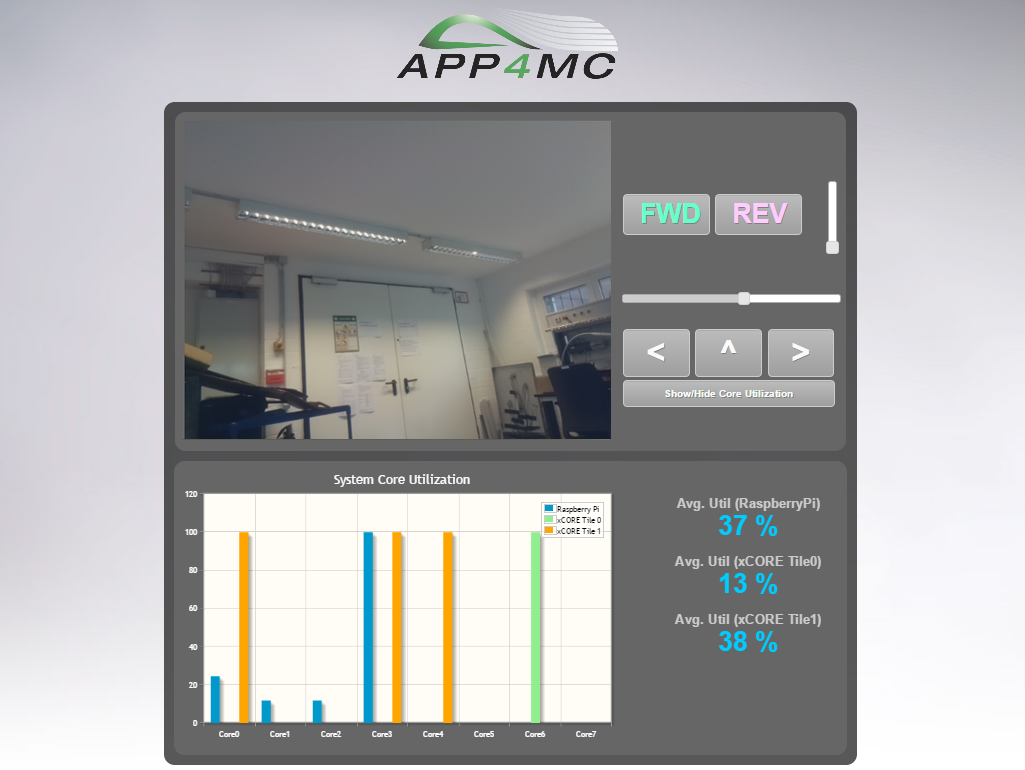
\includegraphics[scale=0.42]{content/images/web.png}
	\caption{Web interface of A4MCAR}
	\label{fig:web}
\end{figure}
%Very briefly but include technologies and how it works, jquery-ajax, html,css and so on.
\subsubsection{Controlling A4MCAR via Web Page}
Some text will come here! \\
\subsubsection{Camera Streaming}
Some text will come here! \\
\subsubsection{Core Utilization Display}
Some text will come here! \\
\subsection{Dummy Loads}
Some text will come here! \\
\subsection{Image Processing with OpenCV}
Some text will come here! \\
\begin{figure}[!ht]
	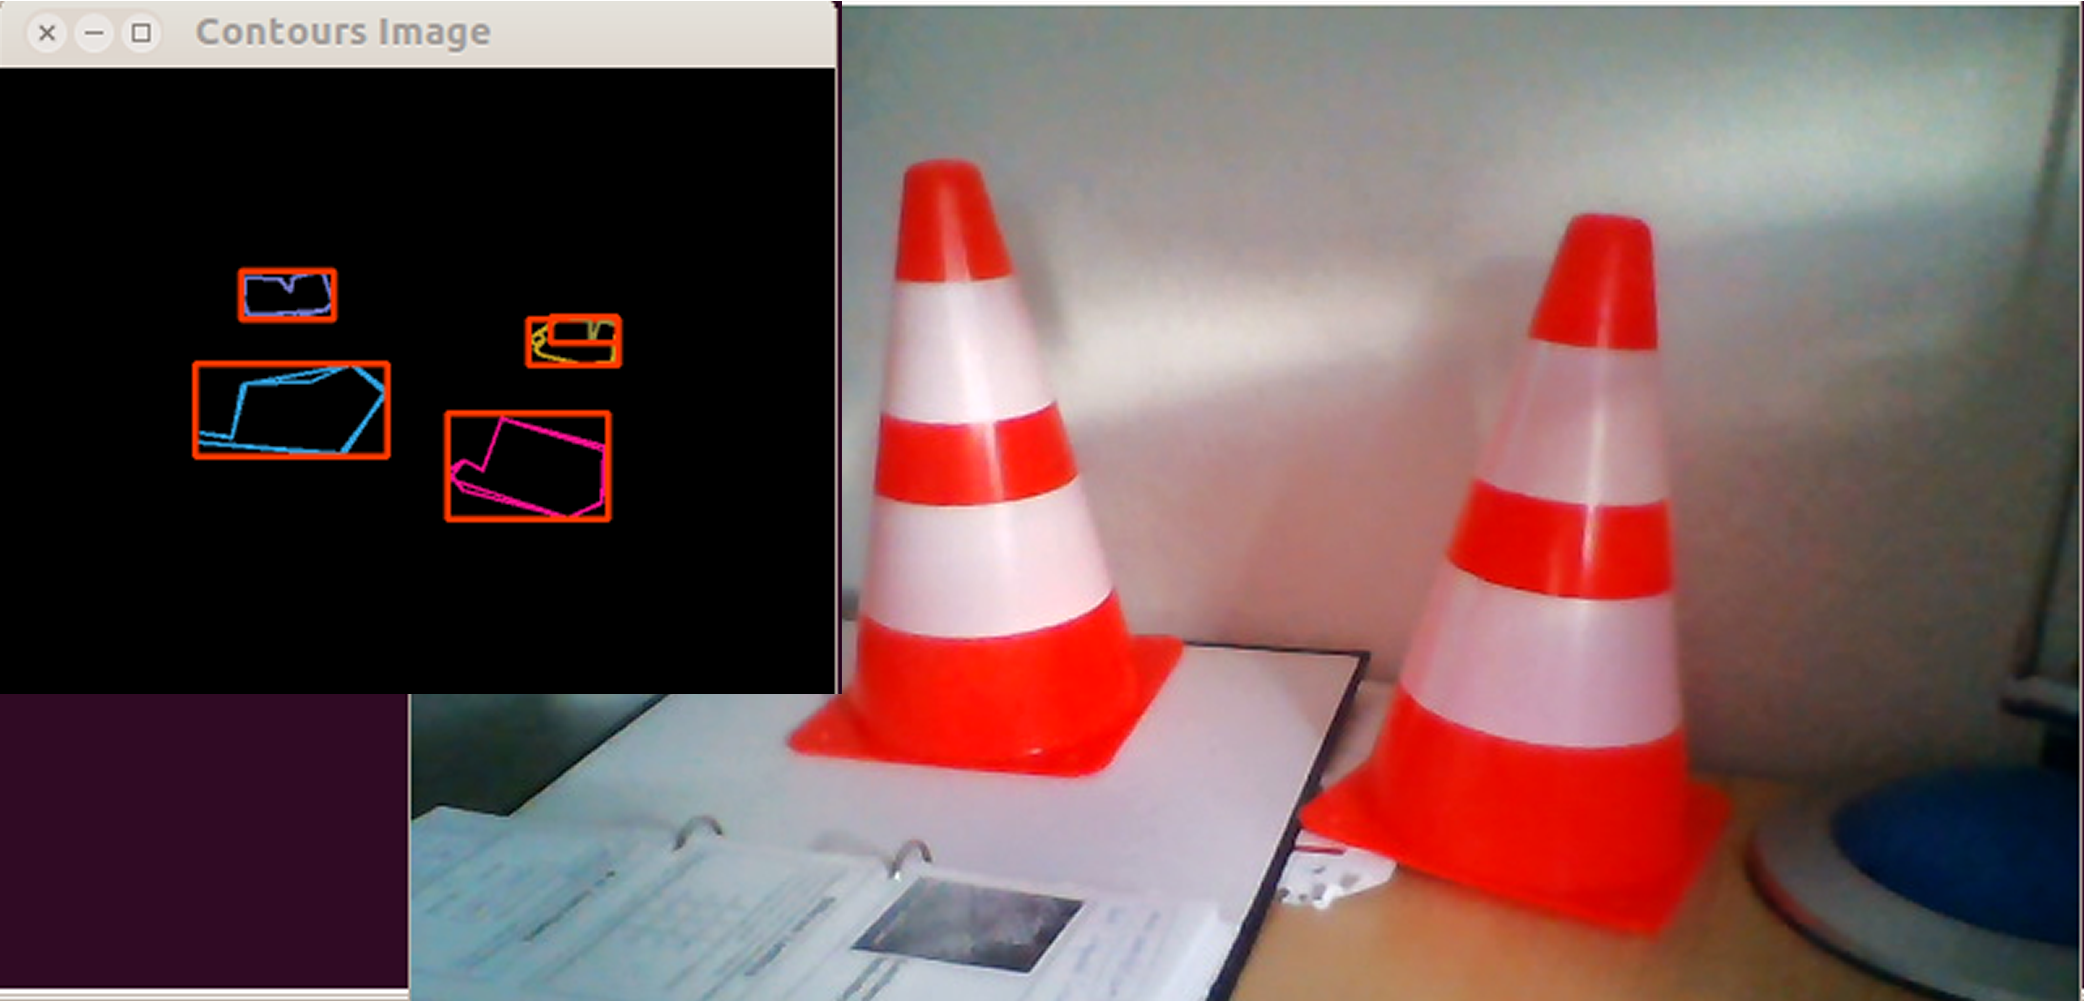
\includegraphics[scale=0.15]{content/images/traffic_cone_detection.png}
	\caption{Developed Image Processing Application}
	\label{fig:traffic_cone_detection}
\end{figure}
\subsection{Touchscreen Display}
Some text will come here! \\
\subsubsection{Touchscreen Display Features}
Some text will come here! \\
\begin{figure}[!ht]
	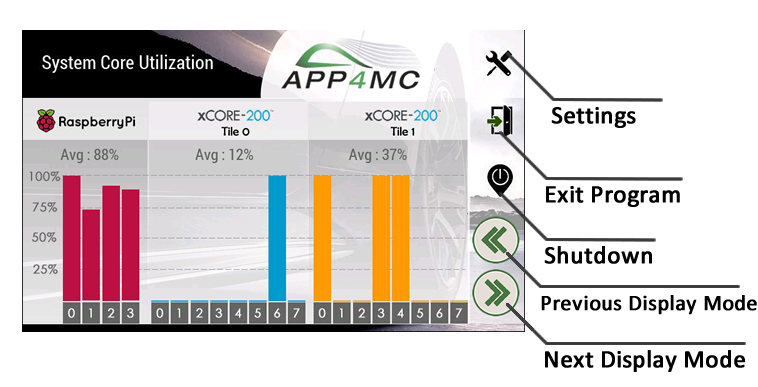
\includegraphics[scale=0.5]{content/images/displaybuttons.png}
	\caption{Button functions of A4MCAR Touchscreen Display}
	\label{fig:displaybuttons}
\end{figure}
\begin{figure}[!ht]
	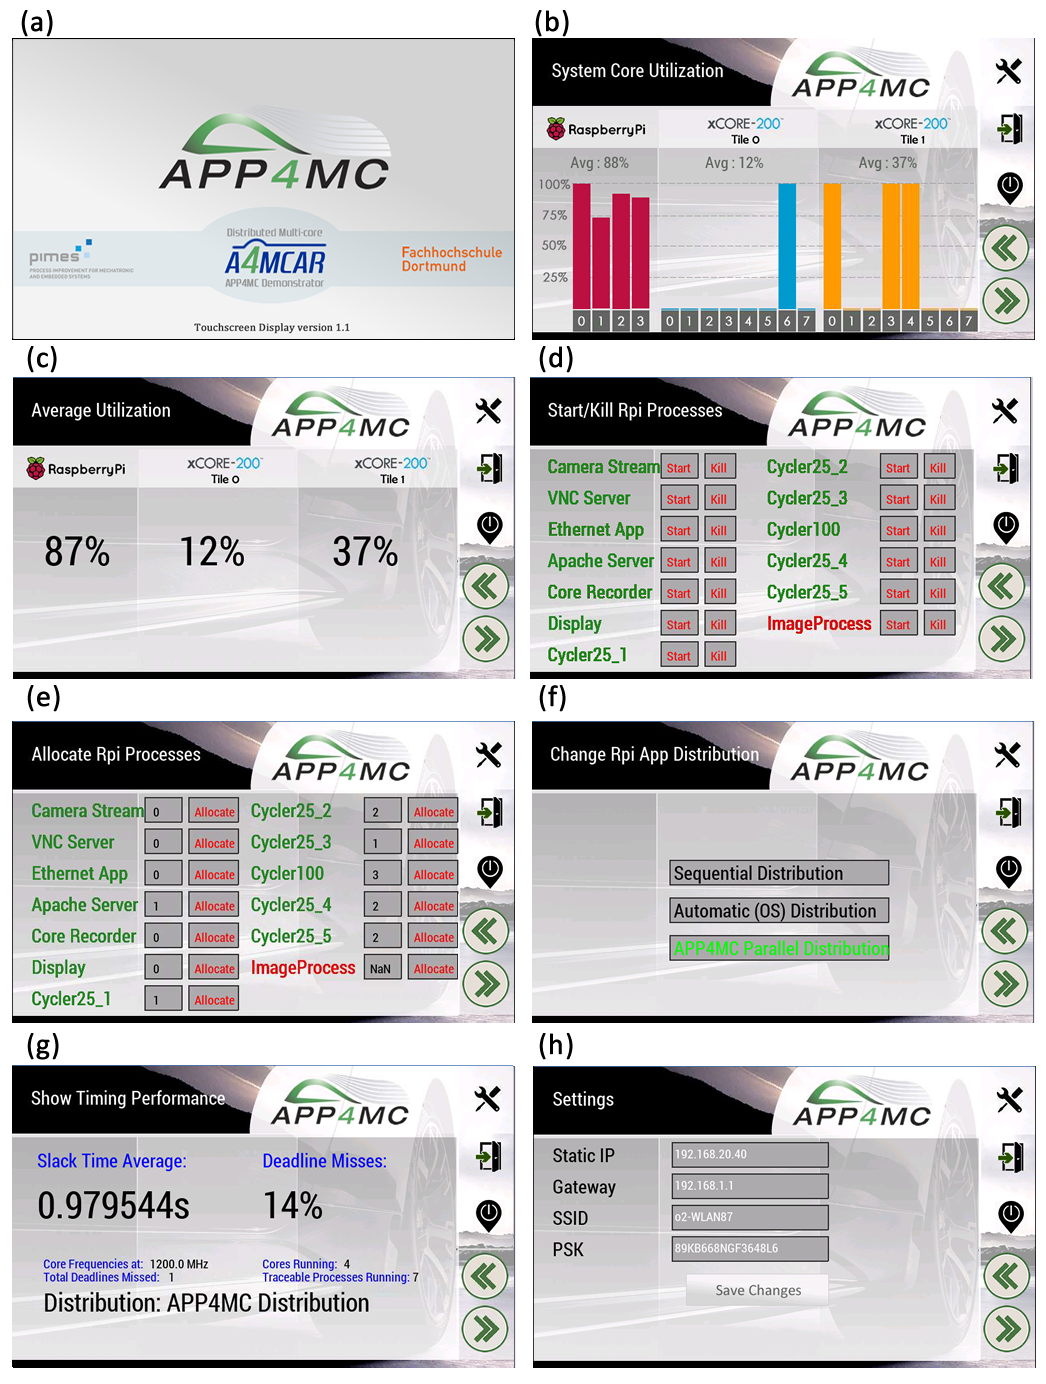
\includegraphics[scale=0.43]{content/images/displays.png}
	\caption{Display modes from A4MCAR Touchscreen Display}
	\label{fig:displays}
\end{figure}
\subsubsection{Touchscreen Display Implementation}
Some text will come here! \\
 %explain used libraries pygame, psutil and touchscreen interfacing hdmi etc...
%Linux tools and created .sh scripts will be in Section (5)
\subsection{VNC Server}
Some text will come here! \\
\subsection{Additional Bash Scripts}
Some text will come here! \\
\section{Android Application Implementation}
Some text will come here! \\
%%% CHAPTER A4MCAR ------------------------------------end----
%%% CHAPTER Information Tracing and System Modeling --------begin----
\chapter{Information Tracing and System Management}
\section{Low-Level Module Information Tracing and System Management}
\subsection{What kind of information needed?}
\subsection{Information Tracing via xTimeScheduler}
\subsection{Information Tracing via APP4MC}
\subsection{Distribution of Tasks to Cores}
\subsection{Discovering Energy Consumption Features}
\section{High-Level Module Information Tracing and System Management}
\subsection{What kind of information needed?}
\subsection{Information Tracing via Linux Kernel}
\subsubsection{Linux Kernel Basics} %processes,threads, scheduling
\subsubsection{top} %including threads
\subsubsection{Process Management using ps Command} % getting pid, getting killing processes
\subsubsection{Using perf to get number of instructions}
\subsubsection{dis}
\subsubsection{objdump}
\subsubsection{Using perf to get scheduling information}
\subsubsection{trace-cmd and kernelshark}
\subsubsection{lttng and TraceCompass}
\subsubsection{proc folder}
\subsubsection{psutil}
\subsection{Distribution of Processes using taskset in Linux}
\subsection{Discovering Energy Consumption Features in Linux with cpufrequtils}


%%% CHAPTER Information Tracing and System Modeling --------end----
%%% CHAPTER Effective Parallelism Evaluation --------begin----
\chapter{Effective Parallelism Evaluation}
\section{Low-Level Module Parallelism} %in RCCAR
\subsection{System Model}
\subsection{Efficiency Model}
\subsection{Evaluation of Different Distributions}
\subsection{Results from APP4MC Distribution}
\section{High-Level Module Parallelism}
\subsection{System Model}
\subsection{Efficiency Model}
\subsection{Evaluation of Different Distributions}
\subsection{Results from APP4MC Distribution}
%Distributed system and embedded systems characteristics.... scalability etc.. real-time system.
%Also description of our systems characteristics.

%x APPSTACLE emphasis
%Quote:
%The main benefit for having release, start, (preemption), end, and deadline values is deriving efficiency. For each task instance, you can calculate e.g. the slack time, that indicates how much time is left before its next execution. The higher the slack time is, the better was its execution. Different scenarios and different tasks have different profiling results (slack time is just one of them) and their investigation leads to a precise assessment of software distribution!
%(Maybe also involve deadline misses..)

%the period usually is the deadline. as soon as execution time exceeds this, you must indicate a “deadline miss” it can lead to system failure or even cause (in the automotive domain) person harm. Think of a break application that must react within e.g. 1ms to ensure accurate braking.
%To answer your question: it is ok, but you must indicate the deadline miss
%you should ‘design’ (since you do not have any timing requirements) the periods in a way that they should meet deadlines
%f you want to show that unser a certain period definition, deadline misses definitely occure (e.g. sequential execution) than you can, for sure, design the periods in that way
% you can measure different scenarios (periods) though (i recommend that)

%Design of rpi apps and timing for real-time scheduling...
%Formulas and how the display timing designed.
%How deadlines designed with periods conforming to parallel distribution

%Linux OS overheads + App Timing additions overhead..


%Give scheduling image.. and explain..

%Real-time Scheduling in Linux?????
%time.time (real time) vs time.clock (processor time) (does not count cpu sleeps)

%Overall mean slack time -> longer means distribution is better.
% Core execution times should be same but Response times  (= GETs ) will slightly differ.
%Why dont we have IPT? which causes Response times = GETs

%Different measurements -> scenerios -> results evaluation using kernelshark, lttng AND TraceCompass!!! and other tools. (also include image processing app in some scenerios)

%Online efficiency calculation using rpi and offline distribution analysis.

% Real-time EMPHASIS REALLY IMPORTANT. MAKE A CHAPTER ON THAT

%Why real-time computing not supported in ARM architecture, especially Raspberry Pi ? (search this!!)

% Thread analizini de yapalim
%top -H -p <pid> or ps -T -p <pid>
%Clock speed > Power

%Problems measuring efficiency using slack time with Rpi:
%There needs to be a dynamic sleep time(period-exectime)
%time.timeshould be used instead of time.clock()

%x DVFS Dynamic Voltage and Frequency Scaling


%%% CHAPTER Effective Parallelism Evaluation --------end----
%%% CHAPTER Conclusion ----------------------------begin----
\chapter{About APPSTACLE Project}
\chapter{Conclusion}

%%% CHAPTER Conclusion ------------------------------end----